\documentclass[thesis.tex]{subfiles}

\begin{document}
\ifSubfilesClassLoaded{
    \setcounter{chapter}{6}
}

\chapter{Estimating transmission} \label{transmission}

In this chapter, I use the estimate of the duration of RT-PCR positivity from combining information from the ATACCC and CIS studies (see \cref{E-imperf-test:sec:conclusion}) to investigate the feasibility of estimating incidence and transmission of SARS-CoV-2 from only the CIS data (described in \cref{E-intro:sec:cis}).
I will show that the CIS data is sufficient; demonstrating the value of surveys of this type for pandemic surveillance.

I take two approaches, backcalculation and a mechanistic model, both previously discussed in \cref{E-inc-prev:sec:infection-process}.

First, in \cref{backcalc}, I use a back-calculation approach, based on \cref{E-inc-prev:eq:EPt}.
This approach enables estimation of incidence within (sub)populations of England.
There are several attractive features about this approach in the context here.
The backcalculation approach makes no assumptions about the transmission process, which have the potential to introduce bias.
It can also easily incorporate arbitrary covariates to adjust for non-response bias.
The scale of the CIS and desire to correct for non-response bias presents challenges for this methodology, especially within the limited computation of the SRS environment.

In \cref{SEIR}, I use a mechanistic compartmental model, within the modelling framework introduced in \cref{E-SEIR:sec:mechanistic-models}.
This approach enables estimating both incidence and components of transmission.
Estimating transmission in addition to incidence answers important epidemiological questions, \eg whether changes in transmission can be explained by changes in contact rates.
I develop a novel observation model to allow the transmission model to be fit to the CIS data.

Finally, in \cref{transmission:sec:comparison}, I compare the results of the two approaches.
I show they give similar values, providing reassurance of the robustness of the results to modelling assumptions.
Overall, there is a bias-variance trade-off between the models.
Fitting to just prevalence data has not previously been done in the literature (see\todo{ref lit review in intro and copy its novelty claims}).

\section{Backcalculation} \label{backcalc}

In this section, I will apply the theory introduced in \cref{E-inc-prev} to estimate incidence.
% First, I explain the method I will apply (\cref{backcalc:sec:methods}) and then present the results (\cref{backcalc:sec:results}).
% I discuss the results in \cref{backcalc:sec:discussion} and conclude in \cref{backcalc:sec:conclustion}.


\subsection{Methods} \label{backcalc:sec:methods}

In \cref{E-inc-prev:sec:observation-process}, I showed that a deterministic approximation to the relationship between true prevalence and incidence is a good approximation for estimating incidence.
This relationship between incidence proportion and prevalence means that once one is inferred, the other is calculated via a deterministic function.
Therefore, a statistical methodology for estimating one of these quantities is required.

Estimation of prevalence from the CIS data was carried out using MRP throughout the pandemic (see \cref{E-biology-data:sec:MRP}).
In this section, I propose extending this process by transforming the posterior distribution of prevalence in each stratum to a posterior distribution of incidence before post-stratifying.

I keep the same logistic regression model in terms of prevalence, transforming its posterior distribution of prevalence to a posterior distribution of incidence.
This results in a two-step process: first, the same inference process described in \cref{E-biology-data:sec:MRP} is used to estimate prevalence; second, the prevalence is transformed to incidence.
An alternative would be an inference procedure that estimates incidence proportion, fit directly to the RT-PCR test results.
This is required to fulfil several desirable features of the model.
Denote the quantity to be inferred (which could be either incidence proportion or prevalence) at time $t$ in strata $i$ as $\pi_{it}$.
The strata will represent at least age group and region, although including ethnicity and sex is also due to non-response in the survey (see \cref{E-intro:sec:cis-strata}).
For many combinations of stratum $i$ and day $t$, the number of positives will be small, often fewer than 5; therefore some form of borrowing between time and strata is required.
The statistical model and inference procedure should have the following properties.
\begin{enumerate}
    \item The smoothing model over time should penalise changes from continuous exponential growth.
        Penalising changes from continuous exponential growth is a natural formulation because mechanistic models predict exponential growth over short periods of time.
        Furthermore, such penalisation has previously been shown to improve estimates of SARS-CoV-2 prevalence by balancing over and under-fitting~\autocite{ealesAppropriately}.
    \item Limit estimates to epidemiologically and biologically plausible values.
        That is, incidence proportion and prevalence should be in the interval $[0, 1]$.
        % While incidence proportion can theoretically be greater than 1, this would imply that some individuals were infected multiple times in a day which is not biologically plausible.
    \item Have sufficient parameters to incorporate all necessary covariates to correct for non-response bias (see \cref{E-biology-data:sec:cis}).
    \item Borrow information across the different covariates.
        The borrowing should penalise towards the distribution of incidence/prevalence across strata in the same geographic region being constant.
        Standard stratified, mechanistic transmission model (such as the one introduced in \cref{E-SEIR:sec:structured-populations}) predict this, if behavioural changes are independent of strata and there is negligible impact of immunity.
    \item Be computationally efficient.
        The model will be fit to granular data and therefore needs to be run within the SRS, with its computational limitations (see\todo{ref section on SRS computational limitations}).
\end{enumerate}

Properties 1 and 2 suggest a model of the form $\logit(\pi_{it}) = g(i, t)$, where $g$ is a function with changes in the first derivative penalised (\ie changes away from linear are penalised).
The $\logit$ link function both limits $\pi_{it}$ to the interval $[0, 1]$, and logit-linear growth approximates exponential growth for small $\pi_{it}$~\autocite{ealesAppropriately}.
Combined with property 4, the form of $g$ the null model is $g(i, t) = a_0 + a_t t + f(i)$ where $a_0$ and $a_t$ are model parameters and $f$ is a function to be specified; that is, changes away from this model should be penalised.
To add additional flexibility, 

% Properties 3 and 4 suggest the extension of the previously-developed MRP method, used to already estimate prevalence, which already satisfies these properties.
% This method has previously been used successfully to estimate prevalence, corrected for non-response bias, from the CIS data~\autocite{cisMethodsONS,pouwelsCommunity,pouwelsMRPvaccination}.


Properties 3 and 5 suggest the use of an approximate method for computing the posterior distribution.
In particular, using MCMC, sufficient covariates to adjust for the non-response bias, and a period of more than 6--8 weeks leads to a model that is computationally prohibitive ~\citePersonalComms{Koen Pouwels}.
Instead, previous MRP implementations have used the Integrated Nested Laplace Approximation (INLA)~\autocite{rueINLA}, implemented in R-INLA~\autocite{RINLA} (see \cref{transmission:sec:INLA}).
theta

\todo[inline]{Is it OK that $x$ and $y$ in the following two paragraphs don't align with the rest of the thesis chapter? Should I use alterantive notation - but then different to standard in the INLA papers.}
INLA-based inference can only be applied to LGMs (\emph{Latent Gaussian Models})~\autocite{rueINLAseminar,rueINLA,martinoINLAtutorial}.
An LGM is defined in terms of a vector of hyperparameters, $\vec{\varphi}$; a deterministic transformation of the hyperparameters into covariance matrix, $\matr{\Sigma}(\vec{\varphi})$; a vector of latent variables, $\vec{x}$; a vector of $n$ data points, $\vec{y} = [y_1, \dots, y_n]^T$; and $n$ linear predictors $\vec{\eta} = [\eta_1, \dots, \eta_n]^T$.
To be an LGM, $\vec{x}$ must be a latent Gaussian field, that is $\vec{x} \mid \vec{\varphi} \dist \N(\vec{0}, \matr{\Sigma}(\vec{\varphi}))$; and the likelihood must have the conditional independence property $p(\vec{y} \mid \vec{\varphi}, \vec{x}) = \prod_j p(y_j \mid \eta_j(\vec{x}), \vec{\varphi})$.

In this context, each element $\vec{y}$ corresponds to the observed RT-PCR results in one stratum on one day.
Hence, $\eta_{j}$ must determine the distribution of $y_{j}$ (up to some hyperparameters); where $j$ can be mapped to a mapping of a stratum $i$ and day $t$.
In practice, this means that $\eta_j$ is a one-to-one transformation of the population prevalence in stratum $i$ on day $t$.
If $\eta_j = \logit(\pi_{it})$, where $\pi$ is prevalence, then a model of $\eta_j = g(i, t)$, as before, is a LGM.
However, if $\pi$ is instead representing incidence proportion, then no such linear relationship between $\eta_j$ and $g$ exists.
In particular, if $\eta_j$ is the prevalence, then $\eta_{it} = \sum_{k=-\infty}^0 \pi_{ik} S(k) = \sum_{k=-\infty}^0 \expit(g(i, k)) S(k)$.
As $g(i, k)$ is linear in the model parameters, $\vec{x}$, then $\eta_{it}$ is not, violating the requirements of a LGM.
Therefore, the application of the INLA approximation, while satisfying the other desirable properties, requires that the regression model predicts RT-PCR prevalence, not incidence proportion.

Next, I explain how I extended the MRP model introduced in \cref{E-biology-data:sec:MRP} to calculate incidence.
I draw a sample of 500 prevalence time series in each stratum from the approximate posterior distribution (using the procedure described in \cref{transmission:sec:INLA:posterior}).
For each stratum, I use the relationship in \cref{E-inc-prev:eq:EPt} to calculate the incidence proportion at each time point.
I consider the relationship between incidence and prevalence within a stratum to be deterministic, as \cref{E-inc-prev:sec:observation-process} justifies, that is the estimate of the incidence is negligibly affected by approximating the distribution $\vec{P} \mid \vec{Z}$ by its mean.
I solve this system using forward substitution, calculating the value of $Z_t$ in \cref{E-inc-prev:eq:forward-substitute} sequentially for $t = 1, \dots, T$.
\Cref{E-inc-prev:eq:forward-substitute} is repeated here for convenience:
\begin{align}
Z_t
&= \frac{P_t - \sum_{i=1}^{t-1} S_{ti} Z_i}{S_{tt}} \\
&= P_t - \sum_{i=1}^{t-1} S(t - i + 1) Z_i.
\label{transmission:eq:forward-substitute}
\end{align}
% \Cref{E-inc-prev:eq:EPt}, considered across different values of $t$, can be written as $\vec{P} = \matr{S} \vec{Z}$, where: $\vec{P}$ is a vector of the number of prevalent individuals at each time point in the stratum; $\matr{S}$ is a matrix formed from the survival function, as defined below; and $\vec{Z}$ is a vector of the incidence at each time point in the stratum.
Dividing each side by the total number of individuals in each stratum transforms number of prevalent individuals to prevalence and incidence to incidence proportion.

Violation of assumptions in various parts of this procedure can lead to the second term in \cref{transmission:eq:forward-substitute} to be greater than the first, giving negative incidence.
In this case, the incidence prior to day $t$ imply that the prevalence on day $t$ is higher than that predicted by the fitted regression model for this strata/day combination.
There are two sets of assumptions which are most likely to be violated.
The first set of assumptions is in constructing survival matrix, $\matr{S}$, which is assumed to be known with no uncertainty in this procedure.
However, \cref{E-imperf-test} showed that the estimate of $S(t)$ is sensitive to assumptions made, such as the assumed $\psens$ and strength of priors used.
The second set of assumptions are in specifying the statistical model used to estimate prevalence, for example the form of the smoothing used.

For $\vec{P} = \matr{S} \vec{I}$ to have a unique solution, $\vec{I}$ and $\vec{P}$ need the same dimension.
However, I am using a period of prevalence which starts after the first infections.
These prior infections will still contribute to the prevalence.
I assume that the incidence up to and including the first day of prevalence data, at $t = 1$, is constant at $I_0$.
Therefore, $P_1 = I_0 \sum_{i=1}^{\dmax} S(i)$ and $I_0 = P_1 / \sum_{i=1}^{\dmax} S(i)$.
For day $t$, the contribution of the incidence for $t < 1$ can be calculated as $P'_t = I_0 \sum_{i=t+1}^{\dmax} S(i)$.
Subtracting $\vec{P'}$ from $\vec{P}$ before applying the forward solving procedure accounts for the contribution of the incidence prior to the first day of prevalence data.

Once the incidence proportion in each stratum has been calculated using this procedure, I poststratify it to the CIS target population and subpopulations of interest.
This is done using the methodology explained in \cref{E-biology-data:sec:MRP}.


\subsection{Results and discussion} \label{backcalc:sec:results}

A slow increase in incidence is estimated to occur over the autumn 2020 period, peaking in late November in most regions (see \cref{transmission:fig:backcalc-regions}).
An exception is the North East and East of England regions (see \cref{transmission:fig:backcalc-regions}(C) and (D) respectively); these regions show no consistent increase or decrease in incidence during October.
All regions then decrease during November; this coincides with the national lockdown which came into force in England on 5th Nov 2020~\autocite{ifgTimeline}.

During November, incidence starts rising, with regional heterogeneity in the timing of when this occurs (see \cref{transmission:fig:backcalc-regions}).
The most explored explanation for this is the emergence of the Alpha variant, which was more transmissible than previous variants and emerged at different times across the country~\autocite{walkerTracking,daviesEstimated,lythgoeLineage}.
There is evidence that when incidence starts increasing is correlated with when the Alpha variant's spread (see \cref{transmission:fig:backcalc-alpha}).
A second peak occurs in late December or early January in all regions; this second peak is larger than the first in all regions except the Northern three (North East, North West, and Yorkshire and the Humber).
\begin{figure}
    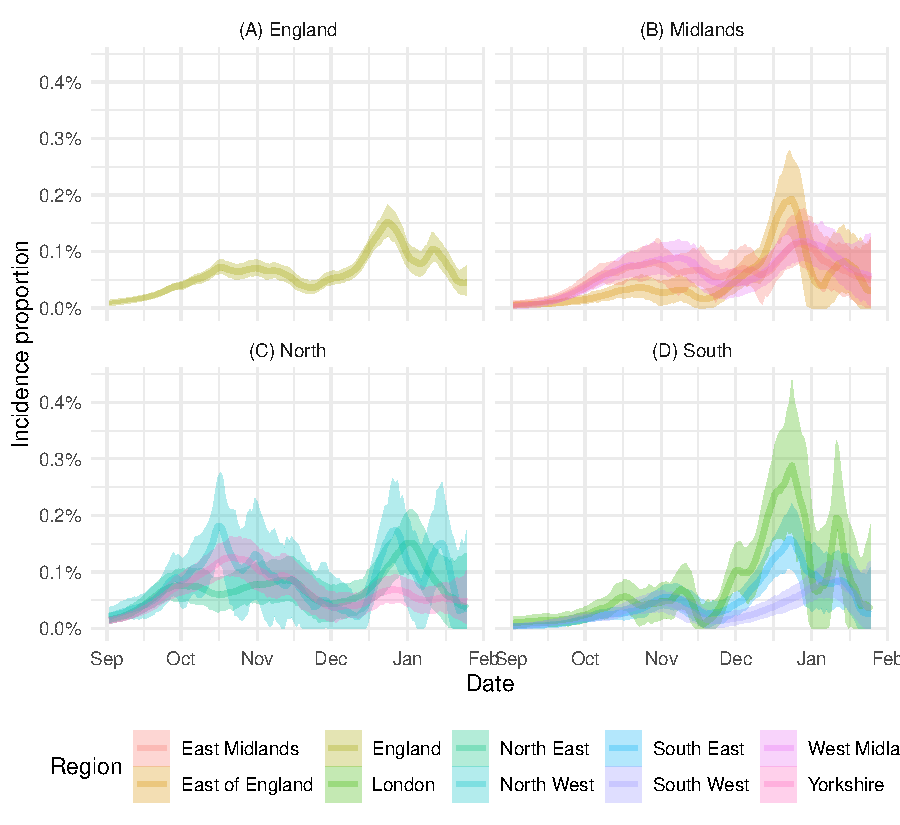
\includegraphics{transmission/backcalc-regions}
    \caption[Incidence estimated using backcalculation by region]{%
        Incidence proportion for all of England (A) and its component regions.
        Regions are split into broad groupings of three regions each: Northern (B), Midlands (C), and Southern (D).
        Yorkshire and the Humber is labelled as Yorkshire for brevity.
    }
    \label{transmission:fig:backcalc-regions}
\end{figure}
\begin{figure}
    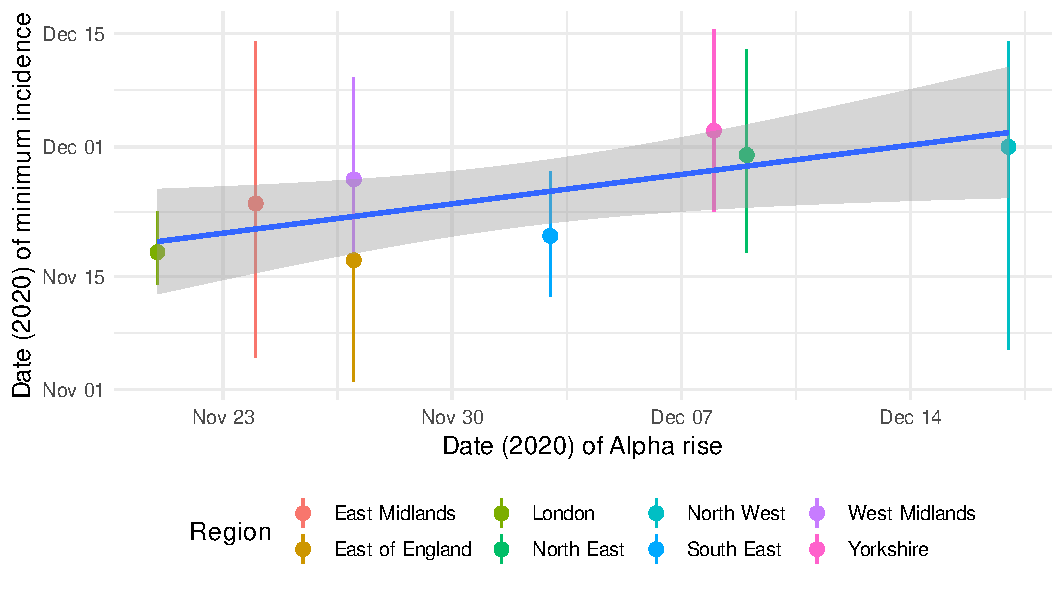
\includegraphics{transmission/backcalc-alpha}
    \caption[Correlation of the emergence of Alpha and minimum incidence.]{%
        x-axis: time that S-gene target failure, a marker of the Alpha variant, is estimated to start increasing from baseline by region among CIS test results; from \textcite[table S3]{walkerTracking}.
        y-axis: posterior median and 95\% CrI of the date of minimum incidence in November or early December in each region.
        Linear regression line shown.
    }
    \label{transmission:fig:backcalc-alpha}
\end{figure}

The incidence proportion was highest among the 11--15 and 16--25 age groups throughout the period (see \cref{transmission:fig:backcalc-ages}).
Except the 16--25 age group, all age groups show similar trends (\ie parallel lines on a log scale), meaning there was insufficient information in the data to overcome the prior which favoured this situation.
The incidence proportion in the 16--25 age group decreases faster than other age groups during November.
There are many plausible explanations for this effect.
The higher incidence in this age group prior to November means it could be an immunity effect.
Alternatively, it could be a consequence of schools remaining open in the November lockdown; 20--24 year olds rarely interact with school-aged children (see \cref{E-SEIR:fig:age-contacts})
Many other explanations are possible, and further work is required to determine causality.
\begin{figure}
    \makebox[\textwidth][c]{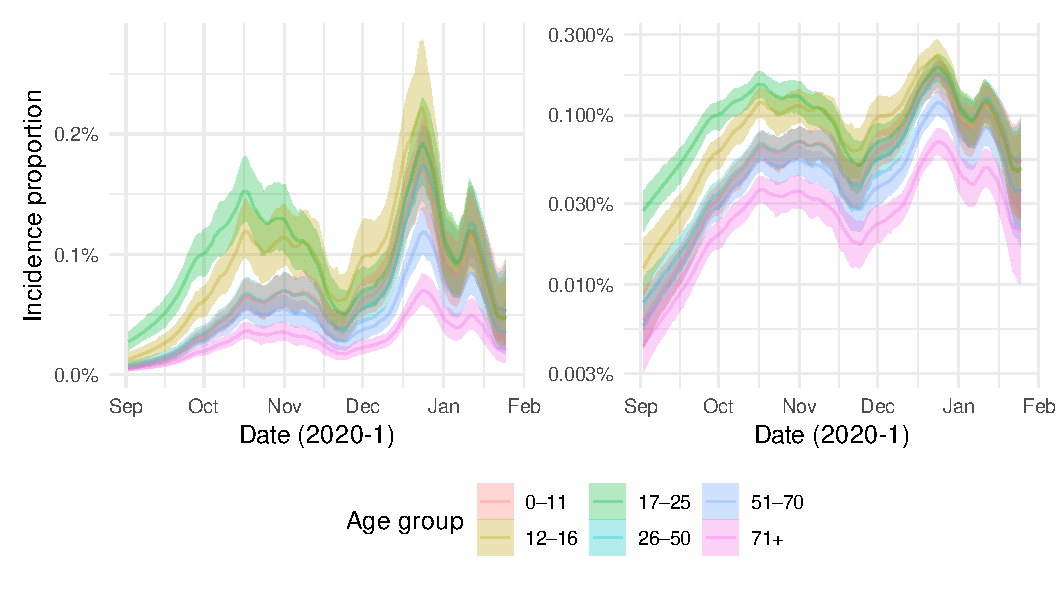
\includegraphics[width=.9\paperwidth]{transmission/backcalc-ages}}
    \caption[Incidence estimated using backcalculation by age group]{%
        Incidence proportion for each age group, on both natural and log scales.
    }
    \label{transmission:fig:backcalc-ages}
\end{figure}

An edge effect where a rapid rise is seen between day 1 and 2 is visible (see \cref{transmission:fig:backcalc-start-effect}).
This is due to the incorrect assumption that incidence is constant in the past.
Changing this assumption (\eg to exponential growth) modifies the estimated value on the first day, but the rest of the series is insensitive to this change (not shown).
Therefore, the first day's estimate is unreliable, and has been excluded from all other plots.
However, the rest of the series is robust to this assumption and hence reliable.
\begin{figure}
    \centering 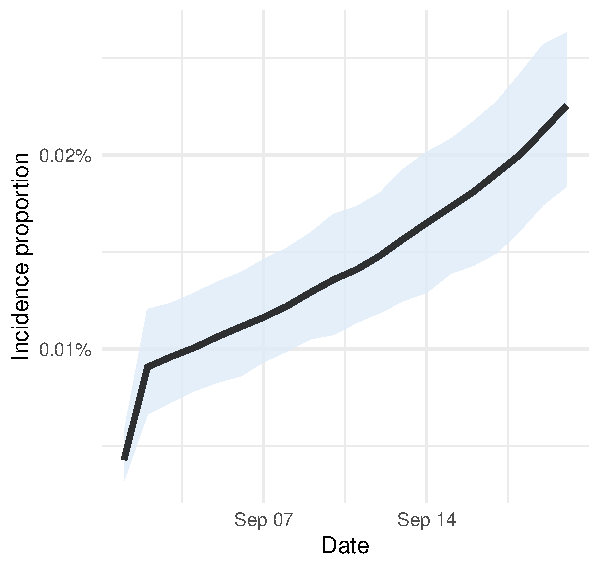
\includegraphics{transmission/backcalc-start-effect}
    \caption[Edge effects in backcalculation method]{%
        First seven days of incidence proportion estimate for the whole of England, highlighting the edge effect.
    }
    \label{transmission:fig:backcalc-start-effect}
\end{figure}

Alternative inference techniques could allow more powerful modelling approaches, if they allowed a broader set of models than LGMs.
In particular, the incidence proportion could be directly modelled rather than the prevalence.
This could allow more interpretable priors to be used because the infection process is the process that corresponds to biological and behavioural processes.
Furthermore, the incidence proportion could be restricted to be non-negative, preventing the negative incidence seen in some strata.

Various alternative inference techniques could be considered.
If the infection process is considered a Poisson process (see \cref{E-inc-prev:sec:poisson-process}), then, conditional on the process's intensity, there is independence between individuals' infection status.
Therefore, the incidence proportion and prevalence can both be viewed as the mean of many Bernoulli variables, meaning that the Central Limit Theorem suggests they are approximately normally distributed.
Exploiting this property could enable efficient approximations to the posterior.


\section{Mechanistic modelling} \label{SEIR}

In this section, I apply the general mechanistic transmission modelling framework from \cref{E-SEIR} to the CIS prevalence data.
The application of this framework follows \textcite{birrellRealtime}, with the most substantial context-specific work\todo{maybe change ``work" to something else: I want a succinct way to say that this was the major part that needed changing from the generic framework in chapter 3} in parameterising the WAIFW matrix (\cref{SEIR:sec:WAIFW-application}).
A novel approach (\cref{SEIR:sec:observation}) links this transmission model to the CIS prevalence data; the approach is generalisable to other studies collecting representative prevalence data, \eg REACT.
In the mechanistic modelling literature, this part of the model is referred to as the observation model, however, in the terminology of \cref{E-inc-prev}, it includes both the prevalence process and the observation process.
Having specified the full model (\cref{SEIR:sec:methods-application}), I conducted a simulation study to validate the inference process and identifiability (\cref{SEIR:sec:sim-study}), before applying the model to the CIS data (\cref{SEIR:sec:application}).
In \cref{SEIR:sec:discussion}, I discuss the results; in \cref{transmission:sec:comparison} I compare the results to those in the previous section.

In common with \cref{E-SEIR:sec:mechanistic-models}, the notation in this section differs slightly from the rest of the thesis.

\subsection{Methods} \label{SEIR:sec:methods-application}

% The model will be stratified only by region and age group, so the data are aggregated to these levels.
% Only individuals aged two or older are eligible to participate in the CIS; I assume that test results in all participants aged under 11 are still representative of the whole $[0, 11)$ age group.

I model each region fully independently, \ie with no shared parameters or transmission between regions.
As well as the motivation given in \cref{E-backcalc}, independent regions allows heterogeneity in the parameters between regions, which could arise from a range of socioeconomic factors.
Furthermore, the assumption of homogeneous mixing within age groups is more plausible for regions than the whole of England.
By modelling each region independently, I assume that the epidemics in each region do not interact.
Clearly, this is not realistic as travel between regions of England is common and unrestricted.
However, except in an epidemic's early stages, the interaction between large regions has a negligible impact on the epidemics progression~\autocite[e.g.][]{birrellRealtimea,gogSpatial,eggoSpatial}.

\subsubsection{WAIFW matrix} \label{SEIR:sec:WAIFW-application}

A parsimonious model is needed to parameterise the WAIFW matrix.
In \cref{E-SEIR:sec:structured-populations}, I explained how the elements of the WAIFW matrix, $\matr{\beta}$ can be decomposed as $\beta_{aa'} = \kappa_{aa'} q_{aa'} N_{a'} / N_{a}$ where\todo{should I repeat these definitions? they already exist in ch 3}: $\kappa_{aa'}$ is the mean rate at which an individual in stratum $a'$ makes contact with individuals in stratum $a$; $q_{aa'}$ is the probability of transmission upon contact between an infectious individual in stratum $a'$ and a susceptible individual in stratum $a$; and $N_{a}$ is the total number of individuals in stratum $a$.
For many epidemics, where the population behaviour is fairly constant over time, a constant $\matr{\beta}$ is a good approximation.
However, in SARS-CoV-2, population behaviour changed dramatically, both spontaneously (\eg due to fear) and in response to government-imposed restrictions.
Therefore, following \textcite{birrellRealtime}, I introduce a time-dependence giving: $\beta_{aa'}(t) = \kappa_{aa'}(t) q_{aa'}(t) N_{a'} / N_a$; $N_a$ and $N_{a'}$ are constant because the change in the total population is negligible over the length of time considered here.

I take information on the contact rates, $\kappa_{aa'}(t)$, from several data sources, using the methodology of \textcite{vanleeuwenTime,vanleeuwenAugmenting}.
%; these estimates have been used for previous modelling of the COVID-19 pandemic~\autocite{vanleeuwenTime,birrellRealtime}.
% These start with estimates of contact in each setting, based on \textcite{vanleeuwenAugmenting}.
This method starts with pre-pandemic baseline estimates of $\kappa_{aa'}$ from the POLYMOD study~\autocite{mossongSocial}, and time use from the UK Time Use Survey (UKTUS)~\autocite{UKTUS}.
POLYMOD asked a representative sample of the UK population about the contacts they make each day, including information on each contact's age and location (home, work, school, leisure, transport, or other).
UKTUS asked a representative sample of the UK population about how much time they spent doing various activities (\eg shopping and spending time at home) each day.
\Textcite{vanleeuwenAugmenting} combined these two datasets to estimate the rate of contacts between age groups during each activity.
\Textcite{birrellRealtime} then modify these contact rates based on measured changes in time use during the pandemic.
These changes are measured using Google mobility data~\autocite{googleCOVID19} and school attendance data~(unpublished).
Google mobility data are based on the location of Android users over time, relative to a pre-pandemic baseline.
The mobility and school data are averaged over a week then used to down or up-weight the number of contacts in each setting, before combining contacts across settings to form $\kappa_{aa'}(t)$.
$\kappa_{aa'}(t)$ is assumed to be piecewise constant, changing only at the start of each week.
For further details see \textcite{vanleeuwenAugmenting} and \textcite[supplementary material]{birrellRealtime}.

The probability of transmission, $q_{aa'}(t)$, needs further decomposition to be identifiable, for the same issue of dimensionality preventing each element of $\matr{\beta}$ being estimated independently (see \cref{E-SEIR:sec:structured-populations} for a full explanation).
I assume that $q_{aa'}(t) = \beta(t) q^\text{susc}_{a} q^\text{inf}_{a'}$ where $\beta(t)$ is a time-varying reference probability of transmission; $q^\text{susc}_a$ is the relative \emph{susceptibility} of stratum $a$, \ie how vulnerable to infection individuals in stratum $a$ are; and $q^\text{inf}_{a'}$ is the relative \emph{transmissibility} of stratum $a'$, \ie how likely individuals in stratum $a$ are to pass on an infection.
These measures include both biological differences, \eg due to differences in immune systems, or behavioural, \eg if infants are less hygienic than adults.

The time-varying component, $\beta(t)$, allows for behavioural changes that impact transmission but are not captured by the contact matrices (\eg mask wearing).
I impose a random walk prior on $\log\beta(t)$ on the weekly timescale, smoothing its value over time.
This prior encodes that behaviour changes smoothly over time.
\begin{align}
    \beta(t) &= \beta_{\tilde{w}(t)} \\
    \log\beta_{w+1} &= \log\beta_w + \sigma_\epsilon \epsilon_w \\
    \epsilon_w &\sim \N(0, 1)
\end{align}
where $\tilde{w}(t)$ is the week number of time $t$, with week 1 being the first week considered.
Two hyperparameters will be inferred: $\beta_1$, the initial value of the random walk; and $\sigma_\epsilon$, the standard deviation of the random walk (see \cref{SEIR:sec:priors}).
$\beta(t)$ is the only time-varying part of the transmission model that is not fixed a priori.
Therefore, in practice, it will also absorb other effects such as any error in $\matr{\kappa}$.

% $K_{ij}$ and $\beta_{ij}$ appear only as a product and therefore are not individually identifiable.
% Normally, $K_{ij}$ is assumed to be known, for example from a previous contact survey~\autocite[such as][]{mossongSocial}.
% Ideally, all the $\beta_{ij}$ terms would be estimated, but there is normally inadequate data to do so, requiring assumptions to be made to reduce the number of parameters~\autocite[65]{keelingModeling}.
% % $\beta_{ij}$ is then estimated, although often with a parsimonious model
% A common assumption is that $\beta_{ij}$ can be decomposed into two independent components such that $\beta_{ij} = \beta \beta^\text{susc}_{i} \beta^\text{inf}_j$.
% For any stratum $i$, $\beta^\text{susc}_i$ is known as the \emph{relative susceptibility} of stratum $i$.

%Now, we assume that $\beta_{ij} = \beta(t) \beta_{ij}$ where $\beta(t)$ is a non-strata-specific, time-varying component representing precautions taken by the population, for example masking; and $\beta_{ij}$ represents a constant probability of transmission from an infectious individual in strata $j$ to a susceptible individual in strata $i$ given contact, which could, for instance, be affected by differential susceptibility to infection for different age-groups.
%We arbitrarily choose one $\beta_{ij}$ to be equal to 1 for identifiability and hence the other $\beta_{ij}$ values are relative to this reference class.

Studies of pre-Alpha SARS-CoV-2 suggest that all individuals have similar infectiousness but that pre-adolescent children are less susceptible than adults~\autocite{chenRole,vinerTransmission}.
Therefore, I set $q^\text{inf}_{a'} = 1$ for all $a'$, $q^\text{susc}_{a} = q_c$ for 0--11 year olds, and $q^\text{susc}_{a} = 1$ for the remaining strata.
$q_c$ can be interpreted as the relative probability that a child is infected (compared to an adult), given contact with an infectious individual.
%$q_c$ is then estimated, although using an informative prior (see \cref{SEIR:sec:priors}).

\subsubsection{Prevalence and observation models} \label{SEIR:sec:observation}

This section  explains the novel observation model approach I propose for fitting to the CIS prevalence data.
This will link the model in the previous section to the CIS prevalence data.

% Here, I extend the system of ODEs to include compartments representing RT-PCR positive individuals.
% The proportion of RT-PCR positive individuals in each strata is then linked to the CIS using a Beta-Binomial likelihood, with the modelled proportion that are RT-PCR positive as the mean of the Beta distribution.
One approach would be to convolve the incidence based on the transmission model with the RT-PCR duration distribution.
Here, the daily incidence proportion for each stratum derived by solving the system of ODEs governing the transmission model (see \cref{E-SEIR:sec:SIR}), and then prevalence calculated using \cref{E-inc-prev:eq:EPt}.
However, this approach is computationally expensive, likely prohibitively so if performed within a MCMC loop.

A computationally cheaper option, which I will take, is to approximate this convolution by adding compartments to the ODEs.
This approach allows an infected, pre-positive compartment, which I denote $p_0$, to be included.
Up until now, this stage of the disease (shown in \cref{E-biology-data:fig:natural-history}) has been neglected, assumed to be of negligble duration.
An advantage of this modelling approach is that it can be included without complications (\eg issues of numerical stability).

$p_0$ increases at the same rate as individuals flow into $e_1$.
These individuals then transition into a set of compartments, $p_1, \dots, p_l$, each with their own transition rate.
I will choose $l$ and the transition rates such that combined length of stay (\ie time from entry in $p_1$ until exit from $p_l$) approximates the duration of positivity distribution estimated in \cref{E-imperf-test}.
This idea extends the technique of having multiple exposed or latent compartments (introduced in \cref{E-SEIR:sec:non-exponential}).
While the use of exponential or Erlang (gamma distributions with integer first parameter) is common in the observation model of compartmental models~\autocite[e.g.][]{overtonEpiBeds}, the use of more flexible phase-type distributions, as here, has rarely, if ever, been used in practice~\autocite{hurtadoGLCT}.
This broader class of distributions allows the model to capture the tail of the distribution, which is important when incidence suddenly decreases.

\Textcite{osogamiClosed} provide a method to construct the compartments, implemented in the mapfit R package~\autocite{mapfit}. 
The resulting compartmental approximation matches the original distribution up to the first three moments.
Applying the package to the posterior mean of the distribution estimated in \cref{E-imperf-test} gives the model in \cref{SEIR:fig:full-model} with the parameter estimates in \cref{SEIR:table:ec-params} (see \cref{transmission:sec:phase-type} for details).
\begin{table}
    \centering
    \begin{tabular}{c c c c c}
        $l$ & $\omega_1$ & $\omega_{2}$ & $\omega_{3}$ & $\pi$ \\
        3 & 0.0820 & 0.126 & 0.0223 & 0.00973  \\
    \end{tabular}
    \caption{Parameter estimates for the EC distribution approximating the posterior mean of the duration distribution estimated in \cref{E-imperf-test}.}
    \label{SEIR:table:ec-params}
\end{table}
% end table of ec params

I link the modelled proportion of individuals that are RT-PCR positive to the data using a beta-binomial likelihood (as discussed in \cref{E-biology-data:sec:clustering}).
If on each day $t$, each strata $i$ is observed to have $y_{at}$ positives out of $n_{at}$ tests, then the likelihood is:
\begin{align}
    \prod_{a,t} \BB (y_{at} \mid n_{at}, \bar{p}_{at}, \rho)
    \label{SEIR:eq:likelihood}
\end{align}
where: $\bar{p}_{at}$ is the mean proportion of individuals in strata $a$ that are RT-PCR positive on day $t$; and $\rho$ is a nuisance parameter controlling the overdispersion of the beta-binomial distribution.
Denoting the proportion of stratum $a$ in state $p_k$ as $p_{ka}(\tau)$, then $\bar{p}_{at} = \int_{t}^{t+1} \sum_{k=1}^l p_{ka}(\tau) d\tau$.

\subsubsection{Model equations and solution} \label{SEIR:sec:full-model}

\begin{figure}
\makebox[\textwidth][c]{
\begin{tikzpicture}[
    node distance = 2.5cm,
    on grid,
    auto,
    ->,>=stealth',
    every state/.style={draw,rectangle},
    ]

    \node[state] (S) {$s$};
    \node[state, right=of S] (E1) {$e_1$};
    \node[state, right=of E1] (E2) {$e_2$};
    \node[state, right=of E2] (I1) {$i_1$};
    \node[state, right=of I1] (I2) {$i_2$};
    \node[state, right=of I2] (R) {$r$};

    \path (S) edge node {$\lambda$} (E1)
          (E1) edge node {$\sigma$} (E2)
          (E2) edge node {$\sigma$} (I1)
          (I1) edge node {$\gamma$} (I2)
          (I2) edge node {$\gamma$} (R);

    \node[state, below=3cm of E1] (P0) {$p_0$};
    \node[state, right=of P0] (P1) {$p_1$};
    \node[state, right=of P1] (P2) {$p_2$};
    \node[state, right=of P2] (P3) {$p_3$};
    \node[state, right=of P3, draw=none] (P4) {};

    \path  (S) edge node {$\lambda$} (P0)
          (P0) edge node {$\omega_0$} (P1)
          (P1) edge node {$\omega_1$} (P2)
          (P2) edge node {$\pi \omega_{2}$} (P3)
               edge [out=-45,in=-135] node[below] {$(1 - \pi) \omega_{2}$} (P4)
          (P3) edge node {$\omega_{3}$} (P4);
    
    \node[draw, thick, inner sep=0.3cm, fit=(P1) (P3), fill=blue!10,opacity=0.2] {};
\end{tikzpicture}
}
  \caption[SEIR model]{SEIR model used for the analysis in this section. The shaded box represents RT-PCR-positive individuals. Shown for a single stratum.}
  \label{SEIR:fig:full-model}
\end{figure}

The remaining details of the transmission model structure follow \textcite{birrellRealtime}.
The transmission model is a SEIR model with two latent and two infectious states.
To form whole of England estimates, each region is modelled independently with the results aggregated, using the poststratification methodology explained in \cref{E-backcalc}.

A diagram of the model for a single stratum is shown in figure \cref{SEIR:fig:full-model}.
The full system of differential equations for each region is below.
\begin{align}
    \label{SEIR:eq:fullODEs}
    \vec{\lambda}(t) &= \beta(t) (\matr{\kappa}(t) \circ \matr{q}) ((\vec{i_1}(t) + \vec{i_2}(t)) \circ \vec{N}) \\
    \frac{d\vec{s}(t)}{dt} &= -\vec{\lambda}(t) \circ \vec{s}(t) \\
    \frac{d\vec{e_1}(t)}{dt} &= \vec{\lambda}(t) \circ \vec{s}(t) - 2\sigma \vec{e_1}(t) \\
    \frac{d\vec{e_2}(t)}{dt} &= 2\sigma \vec{e_1}(t) - 2\sigma \vec{e_2}(t) \\
    \frac{d\vec{i_1}(t)}{dt} &= 2\sigma \vec{e_2}(t) - 2\gamma \vec{i_1}(t) \\
    \frac{d\vec{i_2}(t)}{dt} &= 2\gamma \vec{i_1}(t) - 2\gamma \vec{i_2}(t) \\
    \frac{d\vec{r}(t)}{dt} &= 2\gamma \vec{i_2}(t) \\
    \frac{d\vec{p_0}(t)}{dt} &= \vec{\lambda} \circ \vec{s}(t) \circ \vec{N} - \omega_0 \vec{p_0}(t) \\
    \frac{d\vec{p_1}(t)}{dt} &= \omega_0 \vec{p_0}(t) - \omega_1 \vec{p_1}(t) \\
    \frac{d\vec{p_2}(t)}{dt} &= \omega_1 \vec{p_1}(t) - \omega_{2} \vec{p_2}(t) \\
    \frac{d\vec{p_3}(t)}{dt} &= \pi \omega_{2} \vec{p_2}(t) - \omega_{3} \vec{p_3}(t)
\end{align}
where $\circ$ indicates element-wise multiplication.

I solve the system of ODEs using Euler's method, discretised at timesteps of $\delta t = 1/2$ days.
That is, if $\vec{x}_t$ is the system state at time $t$ for $t \in \{ 0, 0.5, 1, \dots \}$ then $x_{t+\frac{1}{2}} = x_t + (d\vec{x}(t)/dt) \delta t$.

The mean prevalence on day $t$, used for the likelihood (see \cref{SEIR:eq:likelihood}), can be calculated as $\bar{p}_{at} = \frac{1}{2} \sum_{k=1}^l ( p_{kat} + p_{ka,t+1/2} )$.

\subsubsection{Priors} \label{SEIR:sec:priors}

Priors for the parameters are given in \cref{SEIR:table:priors}.
The parameters governing the duration of positivity ($\omega$s) were explained previously (see \cref{SEIR:table:ec-params}).
The initial conditions and transition rate parameters are unindentifiable in a SEIR model~\autocite{dankwaStructural}, therefore strongly informative priors or fixed values are used for them.
$\sigma_\epsilon$ and $\rho$ are given priors that favour a simpler model.
The prior on $\sigma_\epsilon$ is a penalised complexity prior, favouring a null model of constant values for $\beta(t)$~\autocite{simpsonPenalising}.
The prior on $\rho$ favours a null model of a binomial likelihood.
The remaining parameters have weakly informative priors.
\begin{landscape}
\begin{table}
\begin{tabular}{l c l l}
    Parameter description & Symbol & Distribution & Comment \\
    \hline \\
    Mean latent period & $1/\sigma$ & 3.5 days (fixed) & Based on \textcite{zhaoEstimating} \\
    Mean infectious period & $1/\gamma$ & 4 days (fixed) & Based on \textcite{zhaoEstimating} \\
    Initial proportion without immunity & $\vec\pi$ & See \cref{SEIR:table:immunity-prior} & \\
    Initial proportion infectious & $i^+$ & $\BetaDist(0.5, 1000)$ & Weakly informative \\
    Susceptibility of children & $q_c$ & $\LN(-0.4325, 0.1174)$ & Based on \textcite{vinerTransmission}  \\
    Initial growth rate & $\psi$ & $\N(0.06, 0.04)$ & Weakly informative \\
    Standard deviation of random walk steps on log scale & $\sigma_\epsilon$ & $\Exponential(80)$ & Penalised complexity prior \\
    Overdispersion of observations & $\rho$ & $\Exponential(2 \times 10^5)$ & Penalising deviations from binomial
\end{tabular}
\caption[SEIR model priors]{Priors for each parameter. For details of the distributions and their parameterisations see \cref{E-distributions}.}
\label{SEIR:table:priors}
\end{table}

To form the prior for $\vec{\pi}$, I used the analysis framework of \textcite{amirthalingamSeroprevalence}, applied to seroprevalence data from blood donors~\autocite{amirthalingamSeroprevalence} and a representative sample of children~\autocite{ratcliffeCommunity} in August 2020.
This analysis uses a Bayesian framework to correct the seroprevalence data for the sensitivity and specificity of the serological tests, using an informative prior.
\Textcite{amirthalingamSeroprevalence} formed the prior for the tests by evaluating the tests using samples which are known to be negative (taken before the pandemic) or positive (taken from an individual following a positive RT-PCR test).
A regression model predicts the proportion of the population with prior immunity in each age group and region.
I approximated the posterior of this proportion with a beta distribution to form the prior for the analysis in this chapter (see \cref{SEIR:table:immunity-prior}).
\begin{table}
\centering
\begin{tabular}{l|lllll}
         & $[0,16)$ & $[16,25)$ & $[25,50)$ & $[50,70)$ & $[70,\infty)$ \\
        \hline
        East Midlands & $\BetaDist(8.5, 301)$ & $\BetaDist(18, 256)$ & $\BetaDist(19, 475)$ & $\BetaDist(20, 493)$ & $\BetaDist(5, 337)$ \\
        East of England & $\BetaDist(7.9, 236)$ & $\BetaDist(21, 248)$ & $\BetaDist(35, 677)$ & $\BetaDist(26, 613)$ & $\BetaDist(5.6, 332)$ \\
        London & $\BetaDist(9.7, 131)$ & $\BetaDist(50, 328)$ & $\BetaDist(154, 1331)$ & $\BetaDist(106, 990)$ & $\BetaDist(7.6, 204)$ \\
        North East & $\BetaDist(6.1, 180)$ & $\BetaDist(12, 145)$ & $\BetaDist(14, 274)$ & $\BetaDist(14, 295)$ & $\BetaDist(4.2, 240)$ \\
        North West & $\BetaDist(12, 252)$ & $\BetaDist(38, 353)$ & $\BetaDist(72, 885)$ & $\BetaDist(44, 695)$ & $\BetaDist(6.3, 264)$ \\
        South East & $\BetaDist(8.9, 404)$ & $\BetaDist(17, 319)$ & $\BetaDist(20, 577)$ & $\BetaDist(19, 586)$ & $\BetaDist(4.4, 356)$ \\
        South West & $\BetaDist(6.9, 415)$ & $\BetaDist(11, 277)$ & $\BetaDist(12, 556)$ & $\BetaDist(11, 559)$ & $\BetaDist(4, 492)$ \\
        West Midlands & $\BetaDist(8, 167)$ & $\BetaDist(19, 151)$ & $\BetaDist(32, 475)$ & $\BetaDist(33, 504)$ & $\BetaDist(5.8, 241)$ \\
        Yorkshire and The Humber & $\BetaDist(9.2, 314)$ & $\BetaDist(19, 242)$ & $\BetaDist(27, 589)$ & $\BetaDist(18, 474)$ & $\BetaDist(4.9, 316)$ \\
    \end{tabular}
\caption{Priors for $\vec{\pi}$, the proportion of the population without prior immunity, in each age group and region combination.}
\label{SEIR:table:immunity-prior}
\end{table}
\end{landscape}

\subsubsection{Inference} \label{SEIR:sec:inference}

I compute the posterior distribution using MCMC.
Specifically, I use an adaptive random-walk Metropolis-Hastings algorithm (discussed in \cref{E-MCMC}).
The proposal distribution is a multivariate normal that adapts to the covariance of the posterior.
The adaption algorithm is based on \textcite[algorithm 4]{andrieuTutorial}, with the implementation based on \textcite{ghoshApproximate}'s work.
Proposals are accepted or rejected using the standard Metropolis-Hastings (MH) acceptance probability.
See \cref{SEIR:MCMC-algorithm} for full details.
\begin{algorithm}
 set $\vec{X_0}$ to an initial value of the parameter vector \;
 $\vec{\mu_0} = \vec{X_0}$ \;
 $\matr{\Sigma_0} = \text{diag}(\vec{\mu_0})$ \;
 $\lambda_0 = 1$ \;
 \For{$i = 1, \dots, M$}{
  sample $\vec{Y_}i \sim \N(\vec{\mu_{i-1}}, \lambda_{i-1}\matr{\Sigma_{i-1}})$\;
  set $\vec{X_i}$ to $\vec{Y_i}$ or $\vec{X_{i-1}}$ using a MH acceptance step\;
  update the proportion of proposals accepted so far, $\alpha$ \;
  \eIf(\tcc{No adaptation for 200 iterations}){$i \leq 200$}{
    $\lambda_i = \lambda_{i-1}$ \;
    $\vec{\mu_i} = \vec{\mu_{i-1}}$ \;
    $\matr{\Sigma_i} = \matr{\Sigma_{i-1}}$ \;
   }{
    $\gamma_i = (i - 200)^{-0.6}$ \;
    $\log \lambda_i = \log \lambda_{i-1} + \gamma_i(\alpha - 0.234)$ \;
    $\vec{\mu_i} = (1 - \gamma_i) \vec{\mu_{i-1}} + \gamma_i \vec{X_i}$ \;
    $\matr{\Sigma_i} = (1 - \gamma_i) \matr{\Sigma_{i-1}} + \gamma_i (\vec{X_i} - \vec{\mu_i})(\vec{X_i} - \vec{\mu_i})^T$ \;
  }
 }
 \caption{Algorithm for adaptive random-walk Metropolis-Hastings. $\vec{\mu_i}$ and $\matr{\Sigma_i}$ are an estimate of the mean and covariance of the posterior distribution using information up to iteration $i$. $\text{diag}(\vec{\mu_0})$ is the diagonal matrix with diagonal entries equal to $\vec{\mu_0}$. $\lambda_i$ is the scale parameter of the proposal distribution at iteration $i$, tuned to try and ensure an optimal proportion of proposals are accepted (23.4\%). $\gamma_i$ is the learning rate, which determines how much adaptation occurs. $\gamma_i \to 0$ as $i \to \infty$ so the rate of adaptation is \emph{vanishing}. Vanishing adaptation is required for the algorithm to converge to the target distribution~\autocite[section 3]{andrieuTutorial}.}
 \label{SEIR:MCMC-algorithm}
\end{algorithm}

I transformed parameters with restricted ranges for sampling, to improve efficiency.
Parameters which are constrained to the positive reals ($\sigma_\epsilon$, $\rho$, and $q_c$) were sampled on the log scale.
Parameters which are constrained to the unit interval ($i^+$ and $\vec{\pi}$) were sampled on the logit scale.

I run 4 chains for 1,000,000 iterations each.
The first 500,000 were discarded as burn-in, with the remaining chains thinned to every 100th iteration.
This gives 5,000 posterior samples per region.
This was further thinned to 2,000 samples when calculating posterior predictive quantities (incidence and prevalence) due to their computational cost.

Following \textcite{birrellBayesian}, I reparameterise the model to improve identifiability.
Rather than directly inferring $\beta_1$, I infer the initial growth rate of the epidemic.
In addition, I use a parsimonious parameterisation of the initial conditions using the initial proportion of the population that are infectious and the initial proportion that are susceptible only.
Both of these rely on an assumption that the epidemic is in a steady-state exponential growth phase at time 0 (see \cref{E-SEIR:sec:SIR}).

During such an exponential growth phase, all components of the $\vec{e}$, $\vec{i}$ and $\vec{p}$ compartments grow at the same growth rate, $\psi$.
This follows directly from the ODEs if $\vec{s}$ is constant. 
The growth rate $\psi$ is easily identifiable from the data, and therefore a parameterisation in terms of $\psi$ should be more computationally efficient.
If this is the initial exponential phase, when $\vec{s} \approx 1$, then the basic reproduction number for a SEIR model is linked to this growth rate by~\autocite{birrellBayesian,wearingAppropriate}:
\begin{align}
    \R = \frac{\psi \left( \frac{\psi}{2\sigma} + 1 \right)^2}{\gamma \left(1 - \frac{1}{\left(\frac{\psi}{2 \gamma} + 1 \right)^2} \right)} \label{SEIR:eq:rtoR}.
\end{align}

$\R$ can also be expressed a function of $\matr{\beta}(0)$, and hence $\beta_1$ (as explained in \cref{E-SEIR:sec:structured-populations}).
Combining these expressions, the model can be parameterised by using $\psi$ in place of $\beta_1$ by using the following procedure.
Start by calculating $\R$ from $\psi$ using \cref{SEIR:eq:rtoR}; denote this $\hat{R}$.
$\hat{R}$ is the $\R$ that the current value of $\psi$ implies.
Hence, $\beta_1$ should be set such that $\matr{\beta}(0)$ implies $\R = \hat{R}$.
To do so, define $R^*$ as $\R$ $\beta_1 = 1$.
Using the results of \cref{E-SEIR:sec:structured-populations}, $R^* = D(\matr{\beta}(0)) / \gamma$, computed using $\beta_1=1$ (recall that $D(\matr{\beta})$ denotes the dominant eigenvalue of $\matr{\beta}$).
Finally, set $\beta_1 = \hat{R} / R^*$; as multiplying a matrix by a scalar also multiplies its dominant eigenvalue by that same scalar, this means that $\R$ at time 0 is $\hat{R}$, as desired.

To form a parsimonious parameterisation of the initial state, first focus on the initial proportion of the population that is in the infectious compartments.
Recall, from \cref{E-SEIR:sec:structured-populations}, that in the exponential growth phase, the relative proportion of each stratum that is infectious is proportional to the dominant eigenvector of $\matr{\beta}$, which I denote $\vec{d}$.
Introduce a model parameter $i^+$, the proportion of the population in the $i$ states at time 0 in the strata with the highest proportion infectious.
Define the total number of infectious individuals at time 0 as $\vec{i_0} = \vec{i_1} + \vec{i_2} = \frac{i^+}{\max \vec{d}} \vec{d}$.

From the system of ODEs, the knowledge that all the compartments are growing exponentially at rate $\psi$, and the parameters $\vec{\pi}$ (where $\pi_a$ is the proportion of strata $i$ without immunity at time 0, hence, $\vec{r} = 1 - \vec{\pi}$) one can derive the following for the initial state of the compartments:
\begin{align}
    \vec{i_1} &= \vec{i_0} \left(1 + \frac{2\gamma}{\psi + 2\gamma} \right)^{-1} \\
    \vec{i_2} &= \vec{i_0} - \vec{i_1} \\
    \vec{e_2} &= \vec{i_1} \frac{\psi + 2\gamma}{2\sigma} \\
    \vec{e_1} &= \vec{e_2} \frac{\psi + 2\sigma}{2\sigma} \\
    \vec{s} &= \vec{\pi} - \vec{i_0} - \vec{e_1} - \vec{e_2} \\
    \vec{p_0} &= \vec{e_1} \frac{\psi + 2\sigma}{\psi + \omega_0} \\
    \vec{p_1} &= \vec{p_0} \frac{\omega_0}{\psi + \omega_1} \\
    \vec{p_2} &= \vec{p_1} \frac{\omega_1}{\psi + \omega_{2}} \\
    \vec{p_3} &= \vec{p_2} \frac{\pi \omega_{2}}{\psi + \omega_{3}}.
\end{align}

\subsection{Simulation study} \label{SEIR:sec:sim-study}

I ran a simulation study to check that the inference procedure (\cref{SEIR:sec:inference}) was working correctly and that the model was identifiable.
I ran 100 simulations, with parameters drawn from the priors (see \cref{SEIR:table:priors}) except that the prior on $\psi$ was $\LN(0.048, 0.0035)$.
I used the more informative prior for the simulation study to ensure that the simulations were realistic.
The weakly informative prior, used for the main analysis, allows a wide range of epidemics including some that are shrinking at the start of the time period.
Priors and population sizes were matched to the East of England region, over the same time period as the main analysis.

All other aspects of the simulation model, including $\matr{\kappa}$, are as previously described in this section.
This means that the simulations created realistic incidence and prevalence curves (see \cref{SEIR:fig:sim-data}).
In particular, the October half-term school holiday is visible, especially in the school-age groups and the November lockdown is visible to some extent in all age groups.
\begin{figure}
    \thisfloatpagestyle{empty}
    \vspace{-3cm}
    \makebox[\textwidth][c]{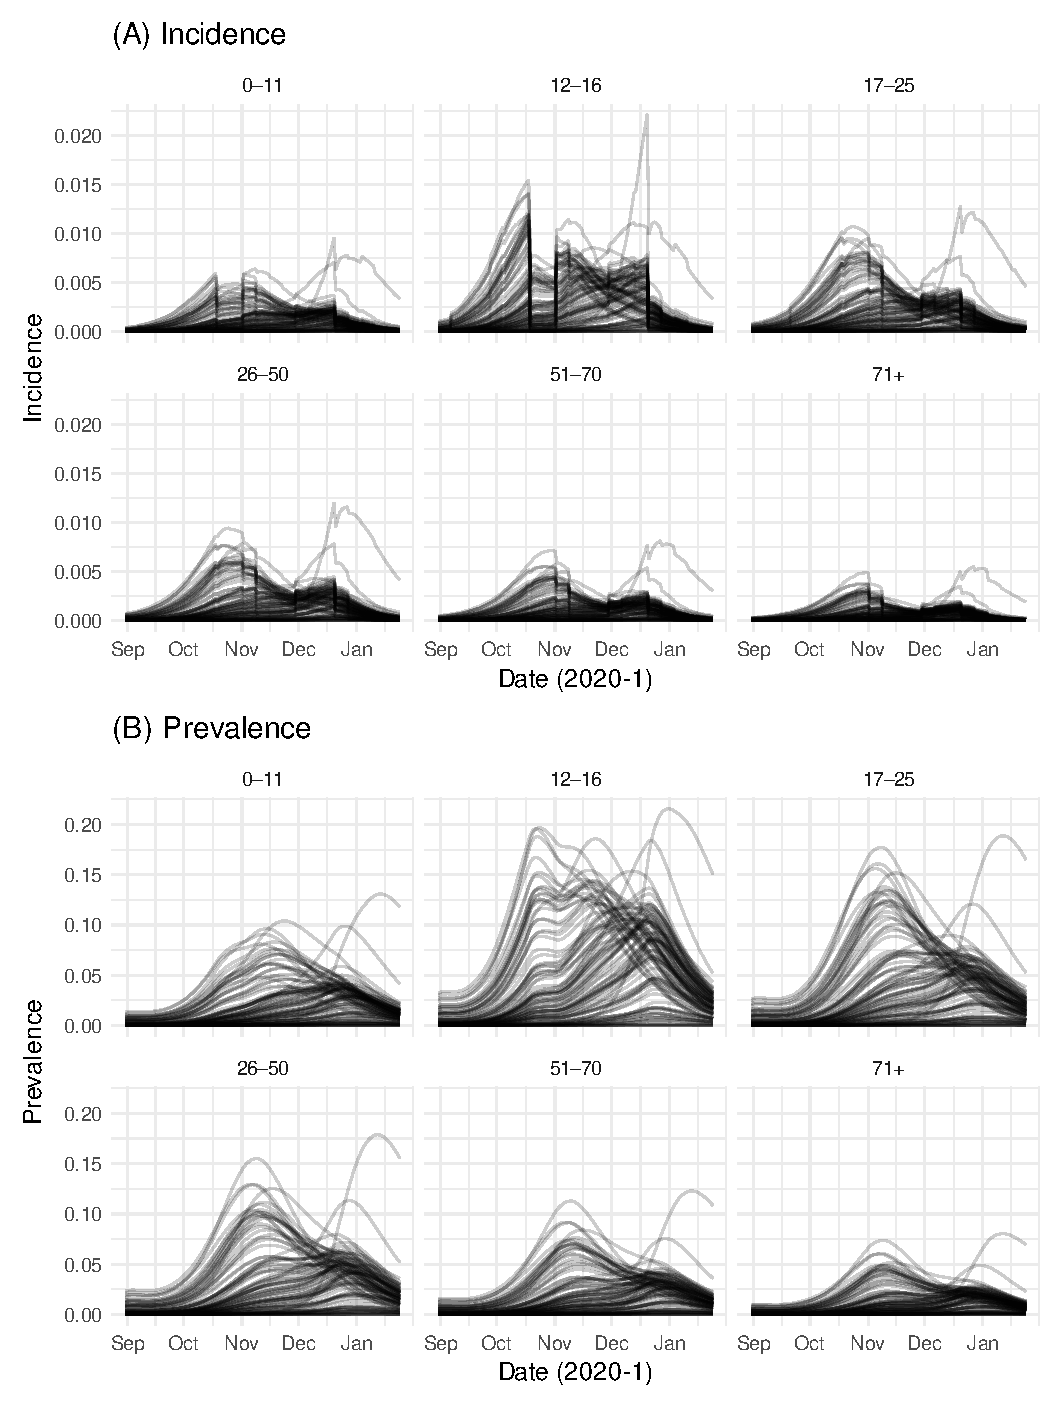
\includegraphics[width=.9\paperwidth]{SEIR/sim/data}}
    \caption[Simulated data]{%
        (A) Incidence and (B) prevalence for the 100 simulated data sets as a proportion of each stratum.
        Prevalence shown is $\bar{p}_{kat}$, the true population prevalence on each day, excluding sampling noise.
        Each line represents one simulation.
    }
    \label{SEIR:fig:sim-data}
\end{figure}

% Furthermore, the combination of the posteriors across all simulations should recover the prior.

To check the performance of the inference procedure, I calculated the coverage of the 50\%, 75\%, and 95\% central credible intervals for each parameter and simulation.
Define coverage as the proportion of simulations where the true value of the parameter in that simulation was within the credible interval.
As the parameters are drawn from the prior, if the inference is performed correctly then the coverage for each parameter should equal the nominal probability (\eg the coverage should be 50\% for the 50\% credible intervals)~\autocite{cookValidation}.
This check is related to, although simpler than, simulation-based calibration~\autocite{taltsValidating}.
I constructed a confidence interval for the coverage using the Pearson-Klopper method implemented in the binom package~\autocite{binom1-1}.

The majority of the confidence intervals contain the nominal probability (see \cref{SEIR:fig:sim-coverage}).
There is a tendency for the coverage to be slightly lower than the nominal probability, suggesting that the credible intervals are slightly too narrow.
This is a common issue with random walk MCMC (see \cref{E-inc-prev:sec:MCMC}).
This is similar when considering coverage of the derived quantities incidence and prevalence (see \cref{SEIR:fig:sim-inc-prev}).
\begin{figure}
    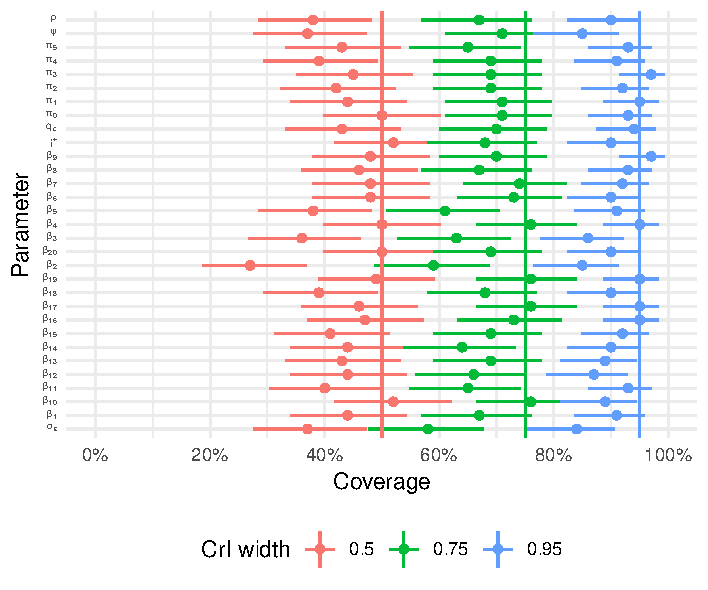
\includegraphics{SEIR/sim/coverage}
    \caption[Coverage of simulation study]{%
        Point estimate and 95\% confidence interval for coverage of the 50\%, 75\%, and 95\% central credible intervals for each parameter; see text for full definition.
        Vertical lines show the nominal coverage.
    }
    \label{SEIR:fig:sim-coverage}
\end{figure}
\begin{figure}
    \thisfloatpagestyle{empty}
    \vspace{-3cm}
    \makebox[\textwidth][c]{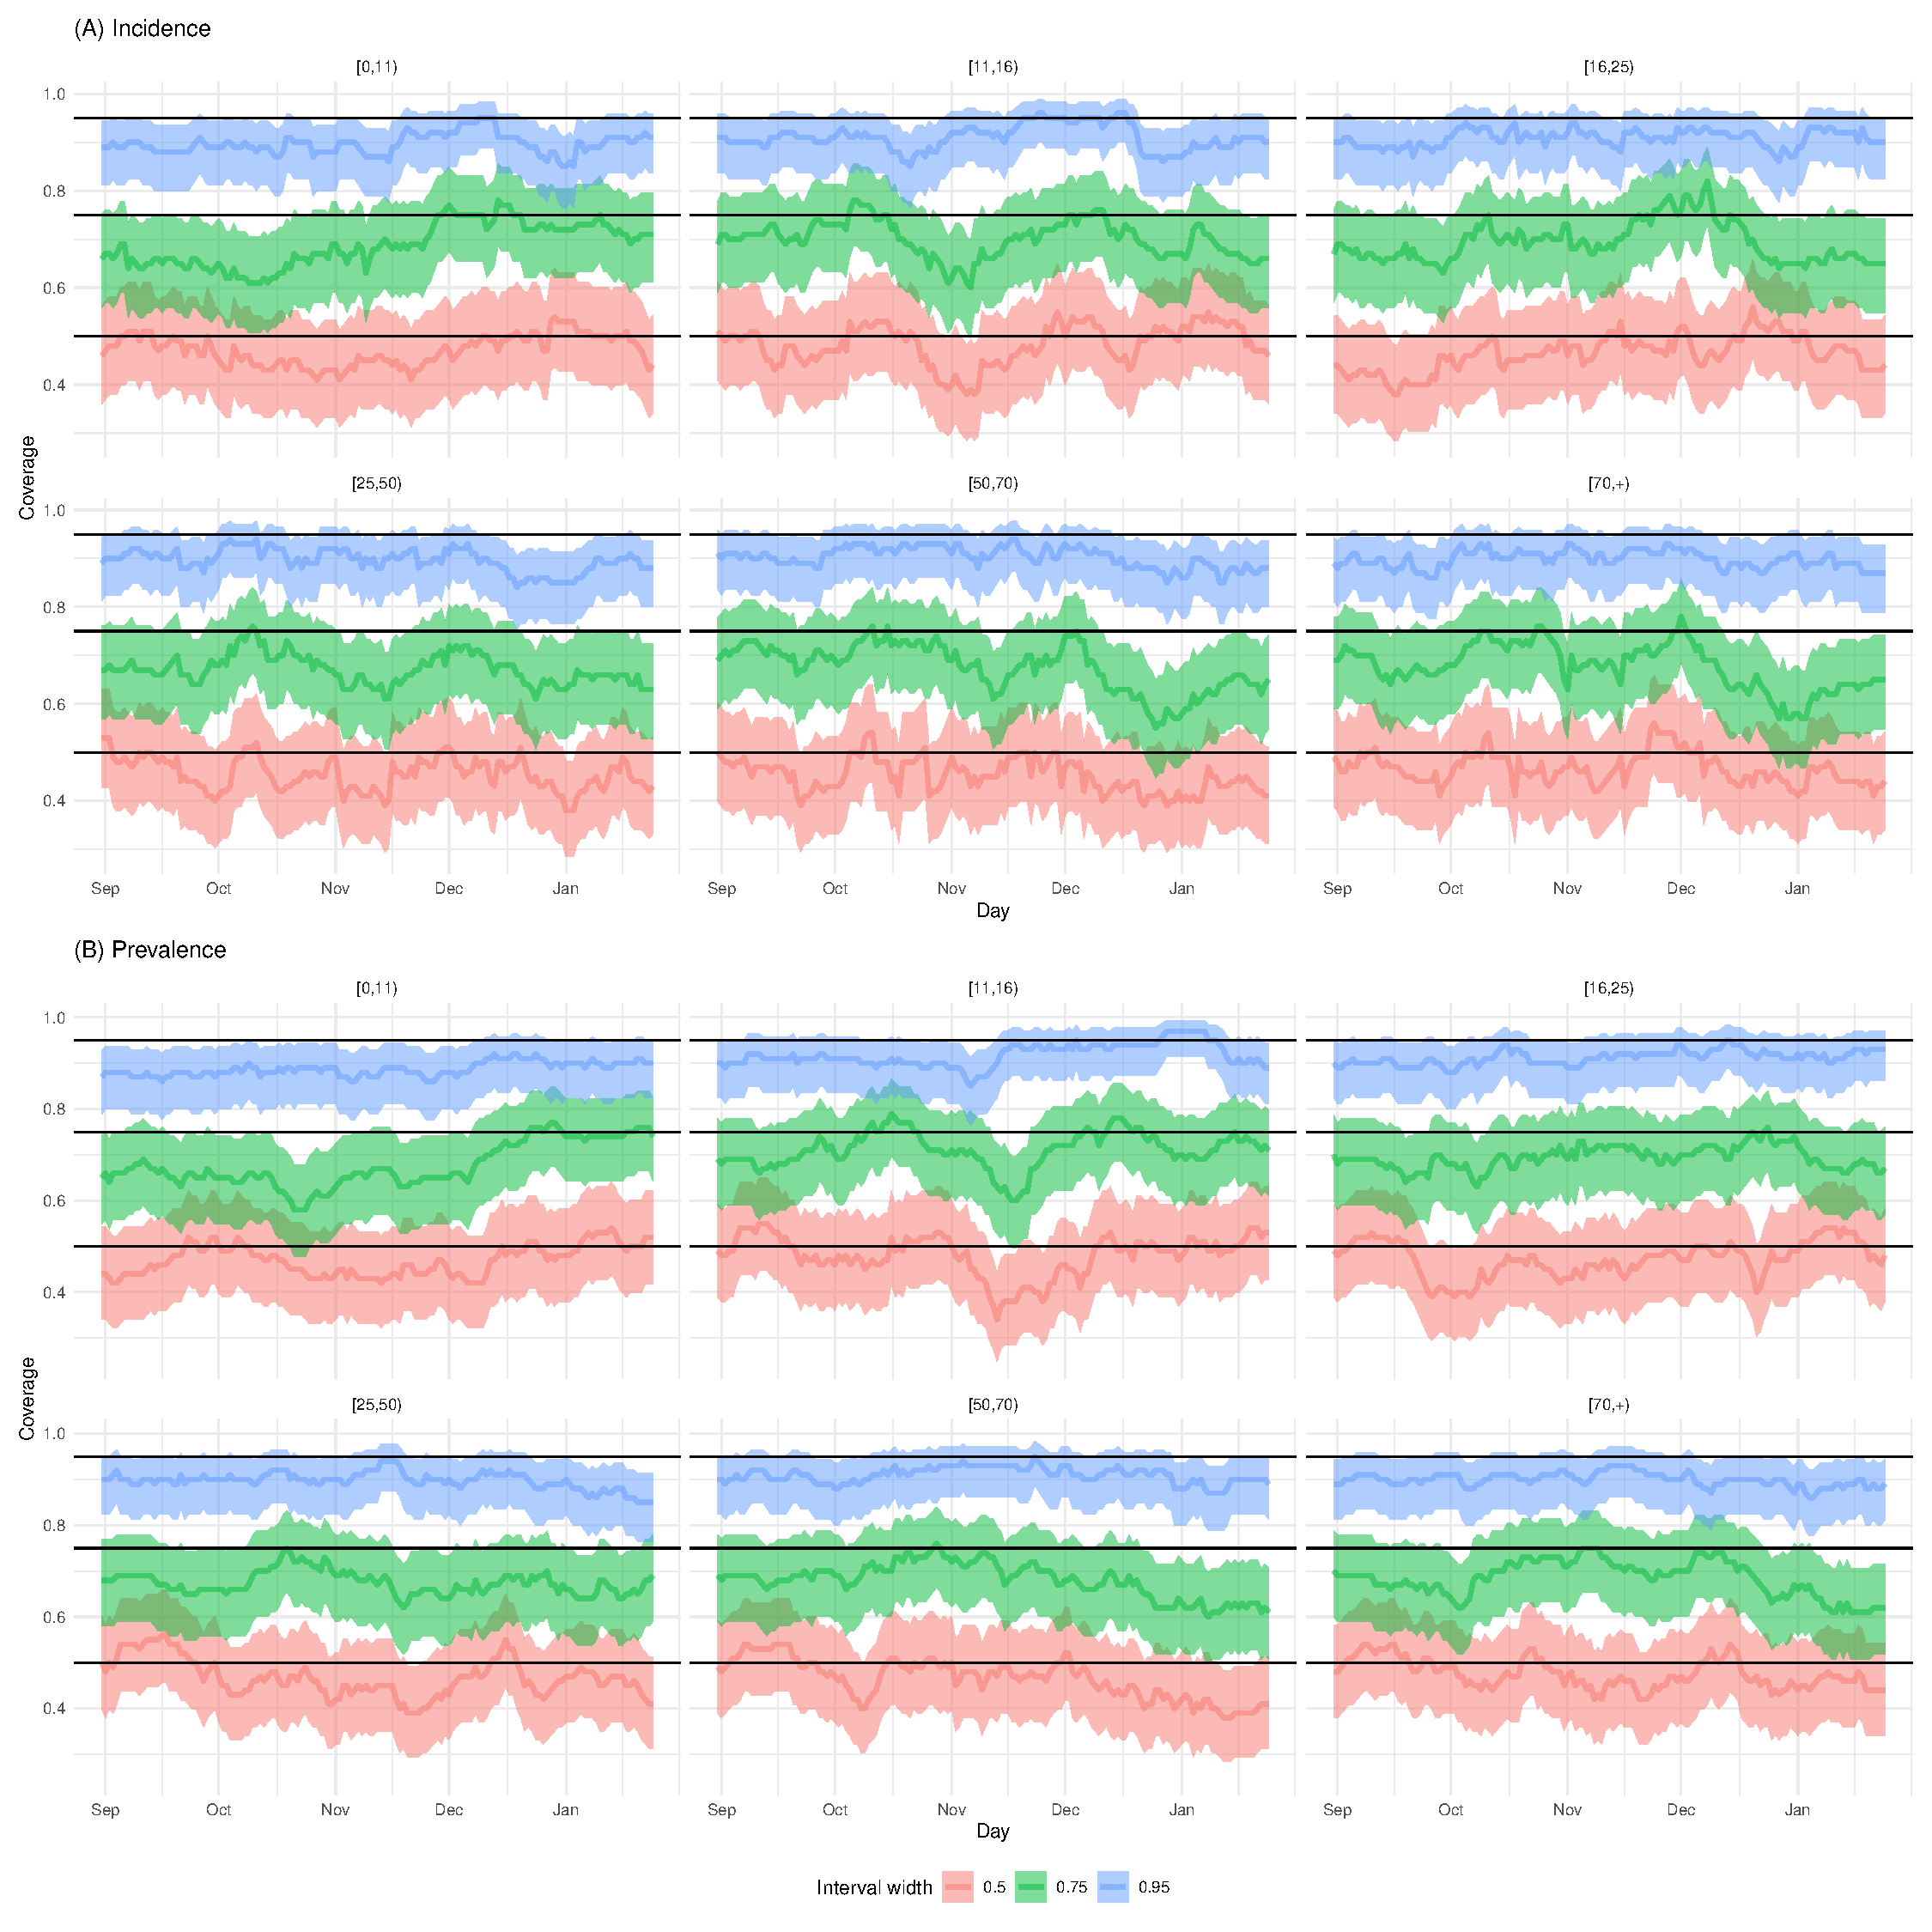
\includegraphics[width=0.9\paperwidth]{SEIR/sim/predictive_coverage}}
    \caption[Coverage of simulation study (derived quantities)]{%
        Point estimate and 95\% confidence interval for coverage of the 50\%, 75\%, and 95\% central credible intervals for (A) incidence and (B) prevalence; see main text for full definition.
        Horizontal lines show the nominal coverage.
    }
    \label{SEIR:fig:sim-inc-prev}
\end{figure}


In this setup, the parameters $i^+$, $q_c$, and $\psi$ are fully identified; $\pi_0$ is not identified at all; the other parameters are partially identified, their posterior has moved away from the prior but is still regularised by it (see \cref{SEIR:fig:true-vs-posterior}).
The ability to identify $q_c$ is an advantage of using data which includes measurements on children, unlike data on hospitalisations or deaths.

For $\vec{\pi}$ and $\rho$, the posterior median is very similar regardless of the true value (see \cref{SEIR:fig:true-vs-posterior}).
This suggests that these parameters are not practically identifiable in this setting.
The posteriors align very closely with the priors (not shown) which reinforces this finding.
The lack of identifiability for $\vec{\pi}$ aligns with previous work showing this parameter is structurally unidentifiable, \ie not identifiable even in the limit of infinite data~\autocite{dankwaStructural}.
\begin{figure}
    \makebox[\textwidth][c]{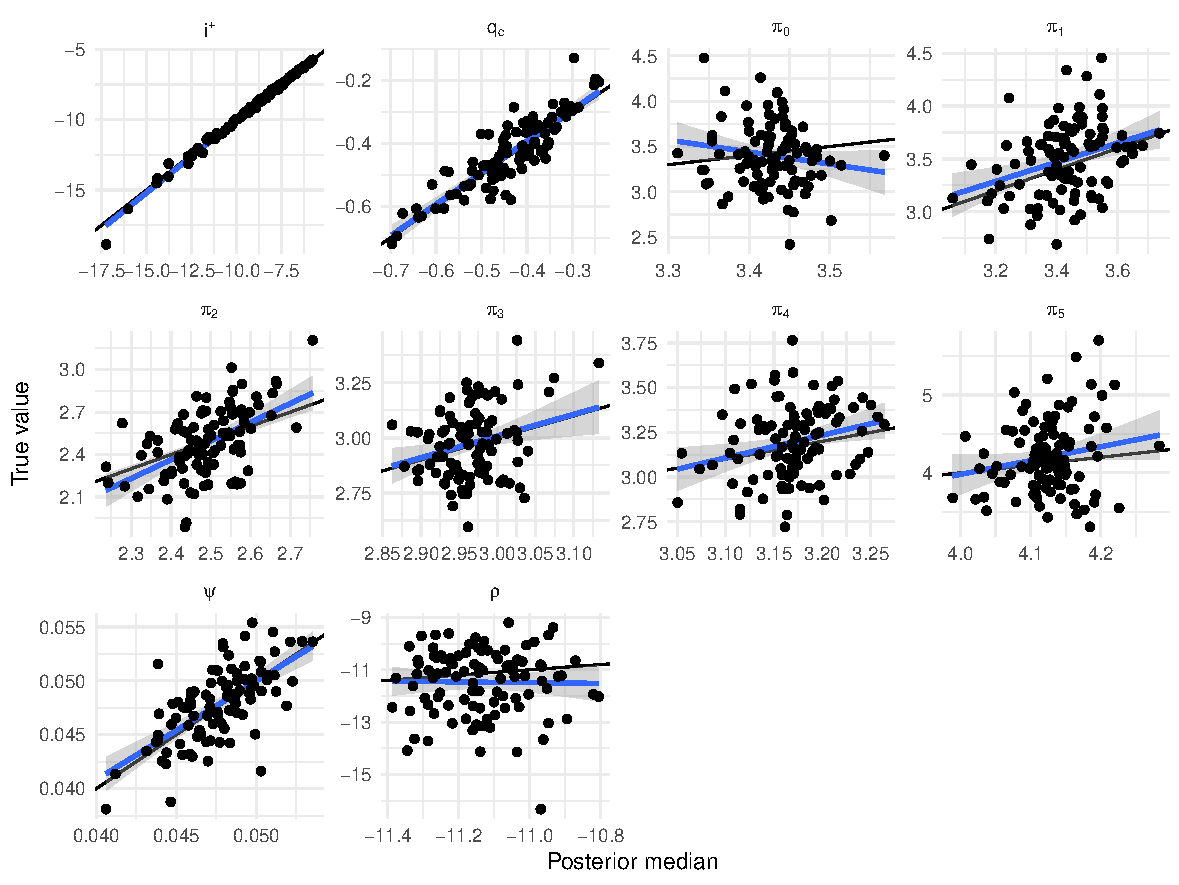
\includegraphics{SEIR/sim/true_vs_posterior}}
    \caption[True vs posterior parameter values]{%
        True vs posterior median parameter values for each parameter in each simulation.
        The black line shows the line $y = x$ which the dots would lie on if the parameter is fully recovered.
        The blue line is a linear regression line.
        For $i^+$, $q_c$, and $\psi$, the posterior recovers the true values.
        For $\vec{\pi}$ and $\rho$, the posterior median is very similar regardless of the true value.
    }
    \label{SEIR:fig:true-vs-posterior}
\end{figure}

\subsection{Application to CIS data} \label{SEIR:sec:application}

The 11--16 age group (roughly corresponding to compulsory secondary school education) is estimated to have the highest incidence (see \cref{SEIR:fig:incidence}).
Incidence is smooth within each week but shows discontinuities between weeks.
This is because the parameters within $\matr{\beta}(t)$ are constant within each week.
A constant $\matr{\beta}(t)$ would lead to exponential growth following a period of transitory dynamics, although the weekly switching may mean that these transitory dynamics never end, especially when incidence is high~\autocite{rhodesConvergence}.
The estimated timing of the peak in incidence varies by region, with the most common time being early January 2021 (see \cref{SEIR:fig:peak-incidence}).
\begin{figure}
    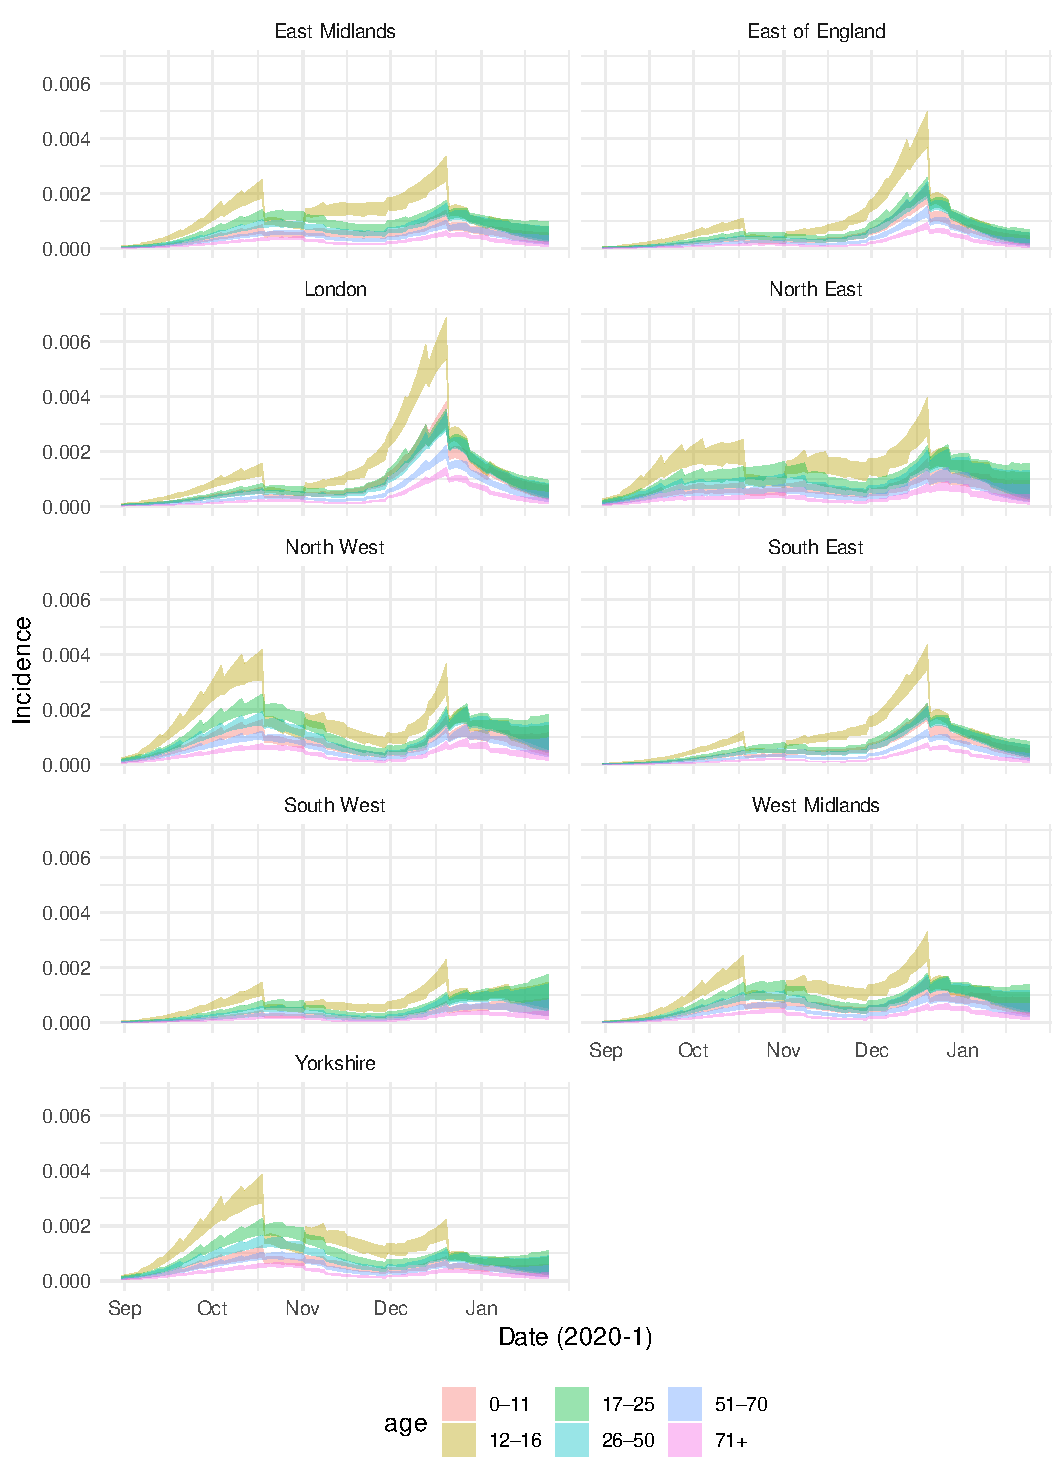
\includegraphics{SEIR/CIS/incidence}
    \caption[Posterior estimates of incidence]{%
        Posterior estimates (95\% CrI) of incidence by region and age.
        See main text for discussion.
    }
    \label{SEIR:fig:incidence}
\end{figure}
\begin{figure}
    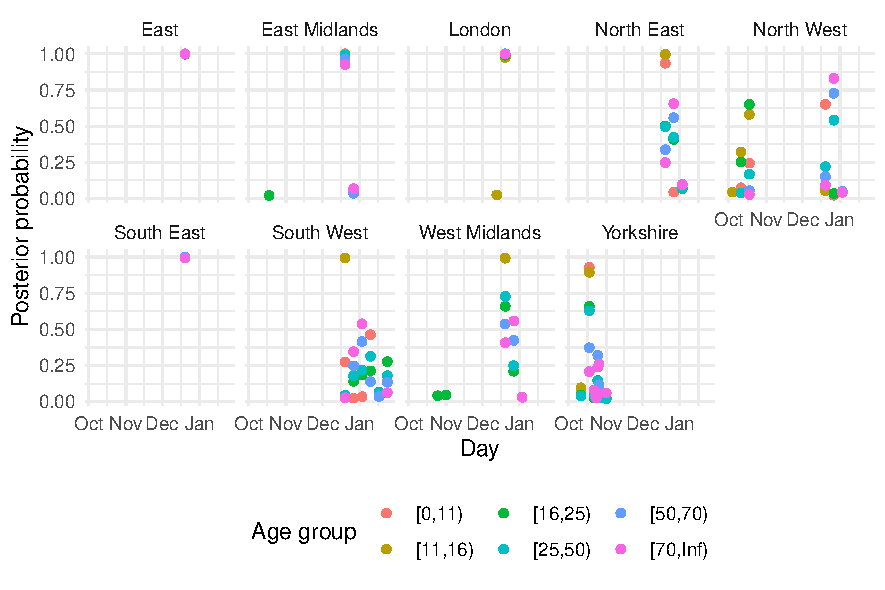
\includegraphics{SEIR/CIS/p_peak}
    \caption[Posterior estimates of peak incidence timing]{%
        Posterior probability of the peak incidence for each region and age combination occurring on each day.
    }
    \label{SEIR:fig:peak-incidence}
\end{figure}

The $\beta_w$ parameters absorb all the time-varying changes in transmission not captured by Google mobility and school attendance data.
They trend downwards up until early December, then they start increasing (see \cref{SEIR:fig:beta-walk}).
Correlation is clear across the regions even though each region is estimated independently, suggesting underlying biological or epidemiological changes across regions as opposed to modelling assumptions.

\begin{figure}
    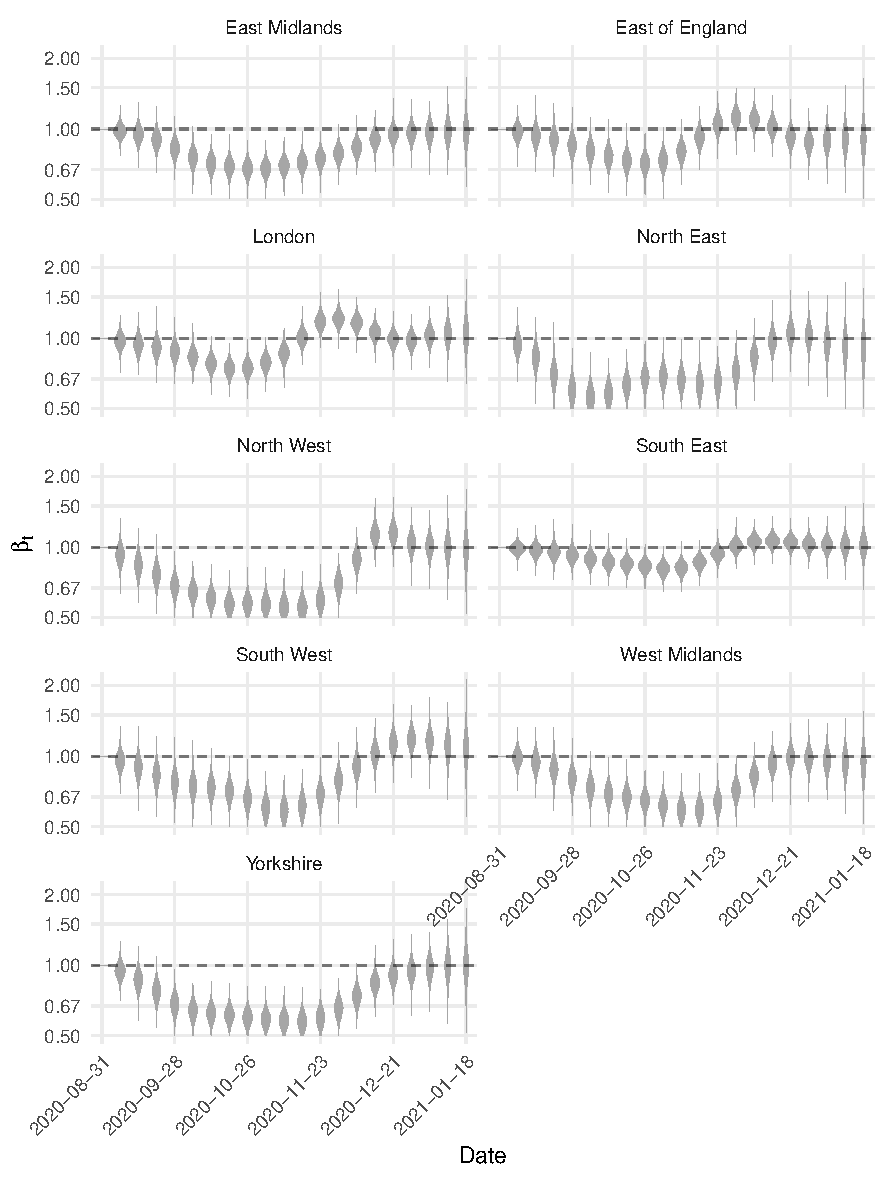
\includegraphics{SEIR/CIS/beta_walk}
    \caption[Posterior estimates of $\beta_w$]{%
        Posterior estimates $\beta_w$ for each week.
        Shown are ``violins'' where the width is proportional to the kernel-density estimated posterior density at that point.
        Values trend downwards until early December when an increase starts.
    }
    \label{SEIR:fig:beta-walk}
\end{figure}

The \emph{attack rate} is the proportion of the population that have been infected at least once.
In this model it is $1 - \vec{s}$, the proportion susceptible.
The attack rate is highest in the $[11, 16)$ age group in the North West at 68\% (95\% CrI: 66--70\%) (see \cref{SEIR:fig:attack-rates}).
Some of these infections occurred prior to the period covered by this study; during this period 23\% (95\% CrI: 21--24\%) of the population in the North West aged 11--16 were infected.
\begin{figure}
    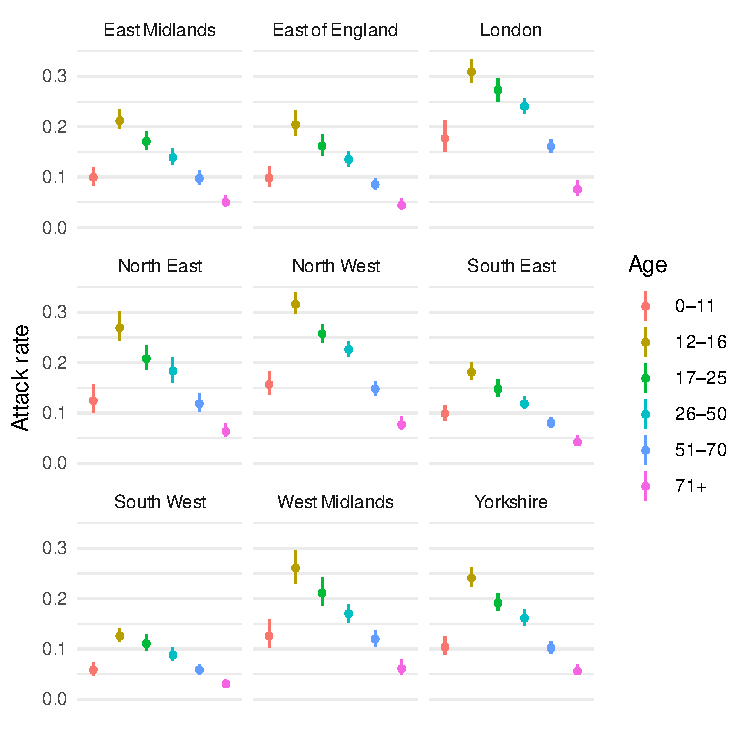
\includegraphics{SEIR/CIS/attack_rates}
    \caption{Posterior median and 95\% CrI of the attack rate in each region and age group.}
    \todo[inline]{Maybe compare this to blood donors, as used in the prior.}
    \label{SEIR:fig:attack-rates}
\end{figure}

Overall the model fits the data well (see \cref{SEIR:fig:prev-young,SEIR:fig:prev-old}).
\todo{move one or some of the goodness-of-fit plots into an appendix - maybe by region?}
There are a few features of the data which are not captured by the model and the posterior estimate appears to be a compromise with the prevalence too low in one age group and too high in another.
For example, in the North East region, the 11--16 age group has its prevalence overestimated in October but the 16--25 age group has its prevalence underestimated.
\begin{figure}
    \thisfloatpagestyle{empty}
    \vspace{-3cm}
    \makebox[\textwidth][c]{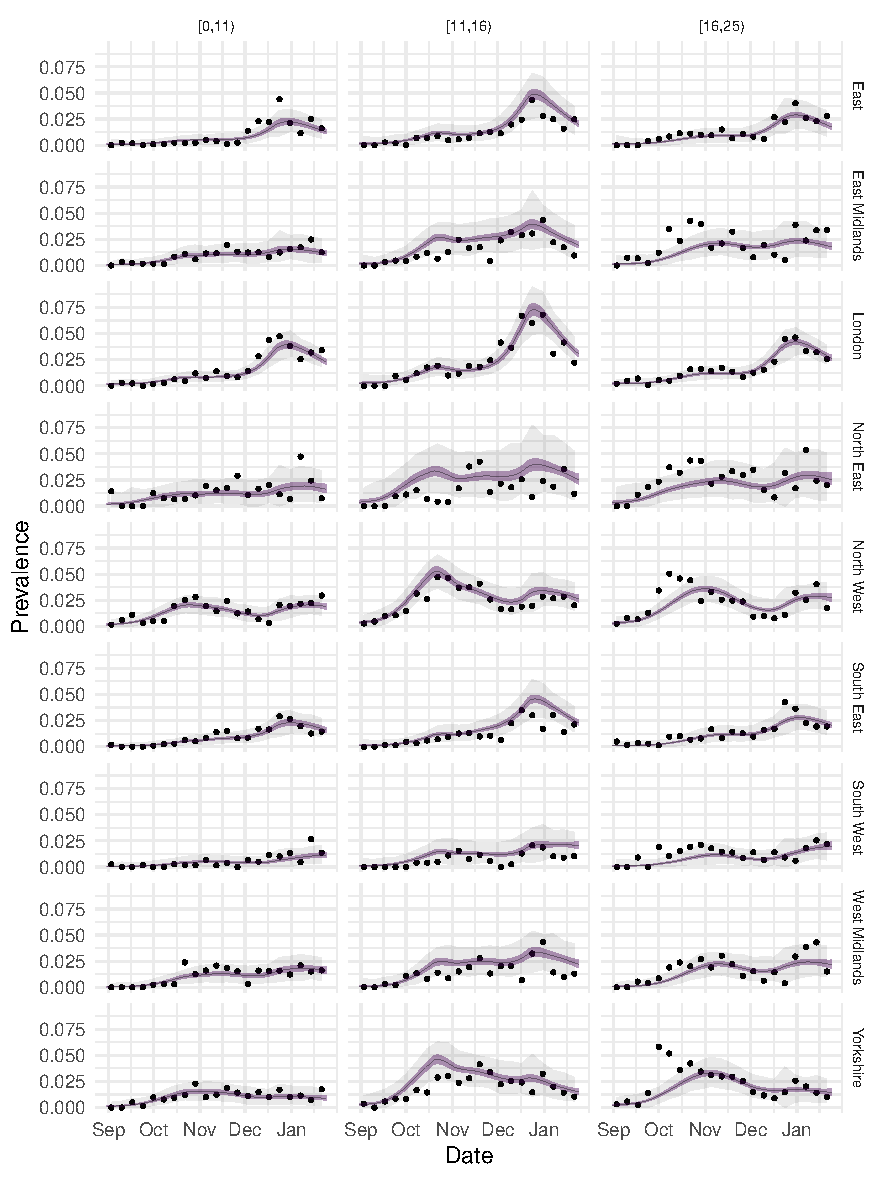
\includegraphics[width=.9\paperwidth]{SEIR/CIS/prev_young}}
    \captionsetup{width=0.8\paperwidth}
    \captionof{figure}[SEIR prevalence goodness-of-fit (younger ages)]{%
        Goodness-of-fit to prevalence data by region and age for the younger three age groups (see \cref{SEIR:fig:prev-old} for the others).
        The central ribbon and line shows the posterior median and 95\% CrI estimate for the proportion of the relevant strata RT-PCR positive on each day.
        The lighter outer ribbon is the 95\% posterior predictive interval for the proportion of test results that are positive each week.
        The dots show the observed prevalence in CIS, aggregated by week.
        For a well-calibrated model, 95\% of the dots would be within the outer ribbon.
    }
    \label{SEIR:fig:prev-young}
\end{figure}
\begin{figure}
    \thisfloatpagestyle{empty}
    \vspace{-3cm}
    \makebox[\textwidth][c]{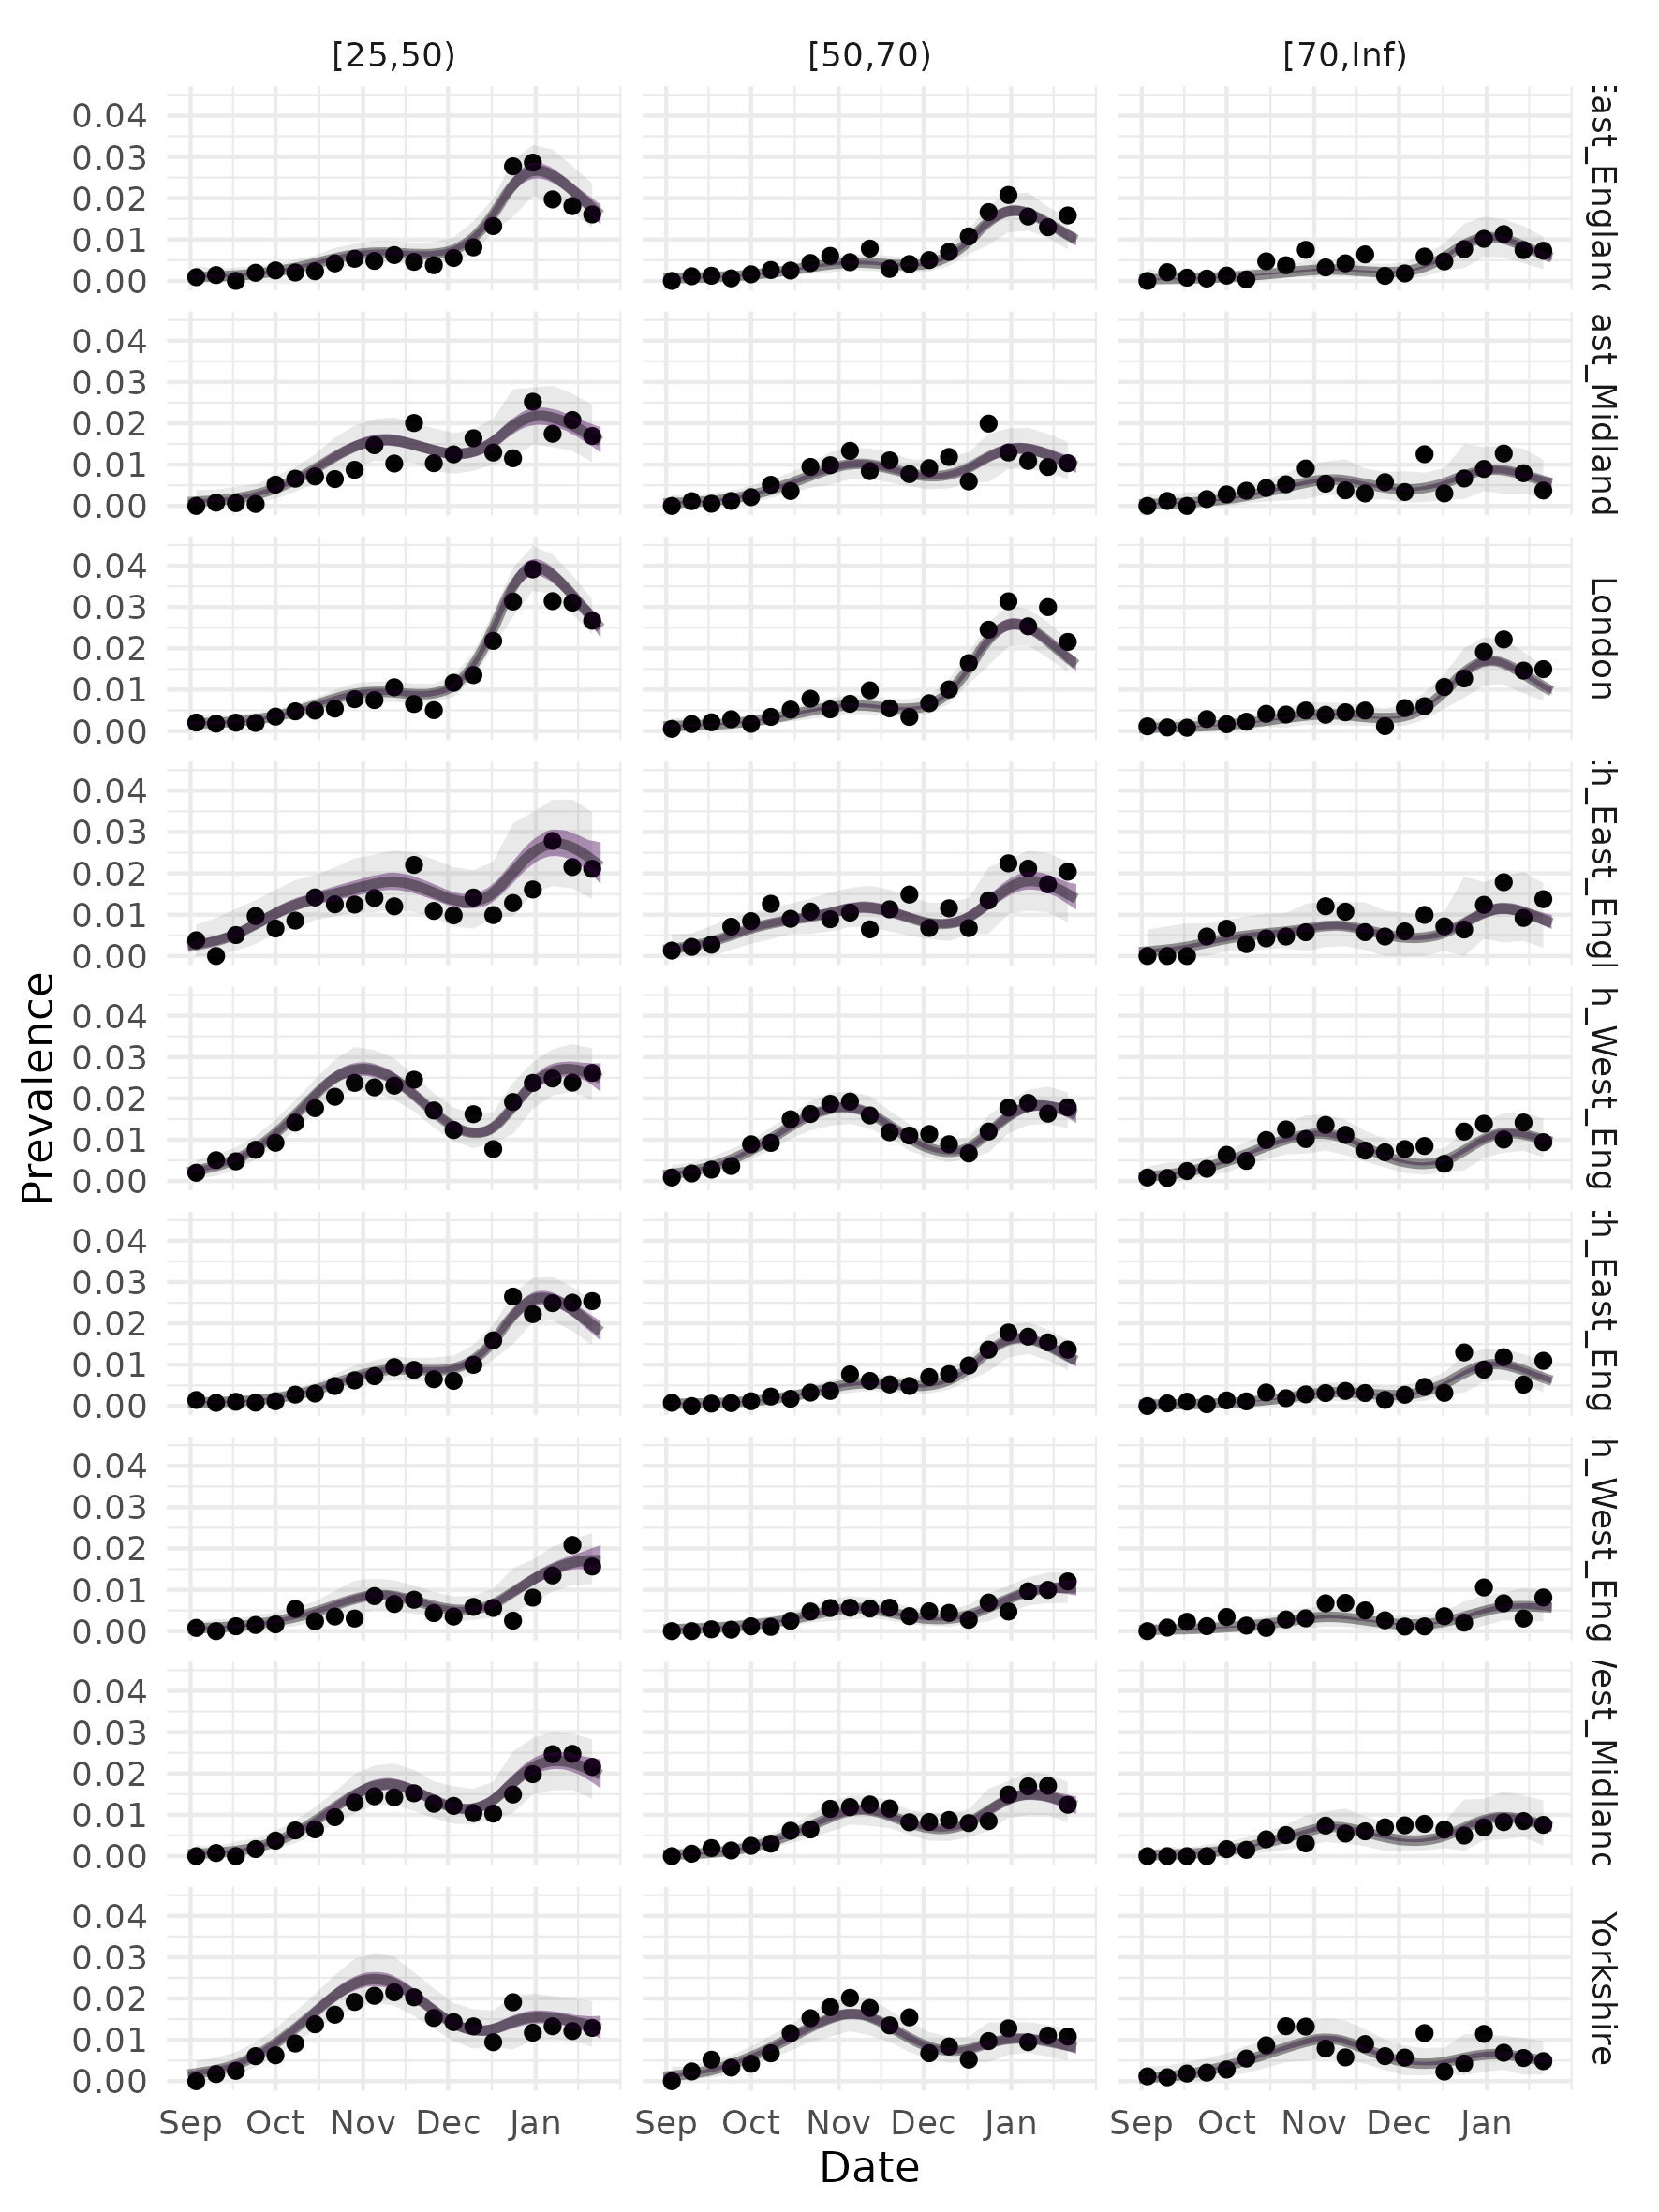
\includegraphics[width=.9\paperwidth]{SEIR/CIS/prev_old}}
    \captionsetup{width=0.8\paperwidth}
    \captionof{figure}[SEIR prevalence goodness-of-fit (older ages)]{%
        Goodness-of-fit prevalence for the older three age groups (see \cref{SEIR:fig:prev-young} for the other age groups and details).
    }
    \label{SEIR:fig:prev-old}
\end{figure}

All regions' MCMC chains converged, assessed using the Rhat statistic and ESS (as defined in \cref{E-intro:sec:MCMC}).
The lowest Rhat was 1.01 for $\sigma_\epsilon$ in London.
All parameters had ESS > 1000, except $\sigma_\epsilon$ and $\psi$ in London, which had ESS of 450 and 950 respectively.

\subsection{Discussion} \label{SEIR:sec:discussion}

The results in this section show the feasibility of fitting a mechanistic model using only data on prevalence.
If the distributions for length-of-stay in each compartment are known, then all other model parameters can  be estimated.
This includes the age distribution of the infections and the components of transmission.

% Unlike most prior work (see\todo{ref section with lit review}), this modelling is based on a data source that is representative of the general population.
% % Therefore, the results have fewer biases and informed by data to a greater extent than this work.
% There is little-to-no ascertainment bias in the CIS, unlike sources relying on testing behaviour (in the UK, pillar 2 testing).
% The CIS allows estimates of transmission in children, unlike sources relying on severe events that occur almost entirely in adults~\autocite{bhopalChildren}.
Using a mechanistic model provides additional understanding, compared to the approach in \cref{E-backcalc}.
For example, decomposing the change in transmission into changing contacts, $\matr{\kappa}(t)$, changing susceptibility $\vec{s}(t)$, and other unmeasured factors, $\beta(t)$.
By understanding which of these components is changing, policies can be better targeted.
If it is shown that $\beta(t)$ decreases, this implies that for a given contact rate in the population, there is less transmission.
Such decreases might be beneficial as it allows society to operate in a more normal manner without increasing transmission.
% Increasing activity without increasing transmission is desirable because it enables reductions the disease burden without burdesome restrictions on individuals day-to-day lives.


The parameters $\beta_w$ absorb all the time-varying factors not captured by Google mobility and school attendance data.
Many factors contribute to the pattern in the $\beta_w$ values, which have a minima near the start of December.
While this analysis cannot establish causation, several hypotheses that are worth considering.

The decreases in $\beta_w$ over the autumn could be due to increased caution (\eg masking or stricter adherence to social distancing) as cases and deaths increased~\autocite{jarvisEffect} and/or not captured by $\matr{\kappa}(t)$, such as the impact of local measures in the highest transmission areas~\autocite{scottCovid19}.
Local measures are not well captured by $\matr{\kappa}(t)$ because the matrix averages behaviour across the whole of England.
Allowing each region to have its own $\matr{\kappa}(t)$ may capture the effect of local measures more accurately, although their targeted nature may require more granular methods.

The increases in $\beta_w$ in December coincide with the rise of the Alpha variant~\autocite{lythgoeLineage}, known to be more transmissible~\autocite[e.g.][]{daviesEstimated}.
A multiple variant model might be able to capture this rise more accurately.
Such a model would stratify positive tests in the CIS by pre-Alpha or Alpha variant.
Then, each variant would be explicitly included in the model to fit to this data.

These hypotheses for the mechanism causing changes in $\beta_w$ are correlated across the country.
This can explain that similar patterns emerge for $\beta_w$ in different regions (see \cref{SEIR:fig:beta-walk}), despite these being estimated independently (\ie there is no model structure which favours correlated values).
These correlations could be exploited to improve the precision of estimates with a more complex model which borrows information across regions, \eg a hierarchical model.

The current model could be more flexible with regards to the age distribution of infections.
This would better exploit one of the strengths of the CIS: the availability of data  on all age groups.
In some regions, there appears to be a trade-off between the 11--16s and 16--25s, with the model misfitting in opposite directions (see \cref{SEIR:fig:prev-young}).
This implies that the data would allow identification of a more flexible age-based model.

Currently, the age distribution of infections is determined by $\matr{\beta}$, and to a lesser extent $\vec{\pi}$, the former of which only contains one parameter that affects the age distribution, $q_c$.
Increasing the number of parameters in $\matr{\beta}$ would be the simplest approach to increase the model's flexibility.

The only time-changing part of $\matr{\beta}$ that varies between ages is $\matr{\kappa}$.
It is plausible that this would not capture all behavioural changes.
For example, the introduction and relaxation of control measures within schools.
$\matr{\kappa}$ only captures changes in in-school transmission through changes in school attendance, not incorporating the probability of transmission, which could be modelled as changes in $q_{aa}$ for $a$ of school age.
Similarly, there is evidence that $q_c$ is different for Alpha and pre-Alpha variants~\autocite{zhuRole}, which could again motivate these changing over time.

The weekly patterns in incidence are a limitation of the current parameterisation.
The random walk and contact matrices both vary only on the weekly timescale.
A daily random walk could provide more flexibility here.
However, this would greatly increase the number of parameters.
An alternative would be a smoothly-varying function or an approximation of a random walk, such as that proposed by \textcite{ghoshApproximate}.

This discussion makes clear that the results are limited by the number of parameters, which is currently limited by the inference algorithm.
The MCMC algorithm used tends to struggle with a large number of parameters.
Alternative proposal schemes, such as updating the parameters in blocks could help, or a more advanced algorithm such as NUTS (used elsewhere in this thesis).

Extending the analyses carried out here to the rest of the pandemic would clearly be of interest.
I chose the end of the period to coincide with the vaccination rollout.
Vaccination dramatically affects the transmission dynamics by introducing some additional immunity into the population.
Mechanistic models require explicit representation of this immunity.

\section{Comparison of results} \label{transmission:sec:comparison}

\Cref{transmission:fig:compare-regions} compares the regional incidence estimates between the two models in this chapter.
Generally the estimates agree, with the SEIR model having much narrower credible intervals.
The largest discrepancy is that the backcalculation model estimates a second peak in mid January in several regions (most clearly in London, North West, and the East of England).
However, except in London, the credible intervals still overlap.
This is a specific case of a larger pattern: the SEIR model produces smoother estimates of incidence than the backcalculation model.;
\begin{figure}
    \centering 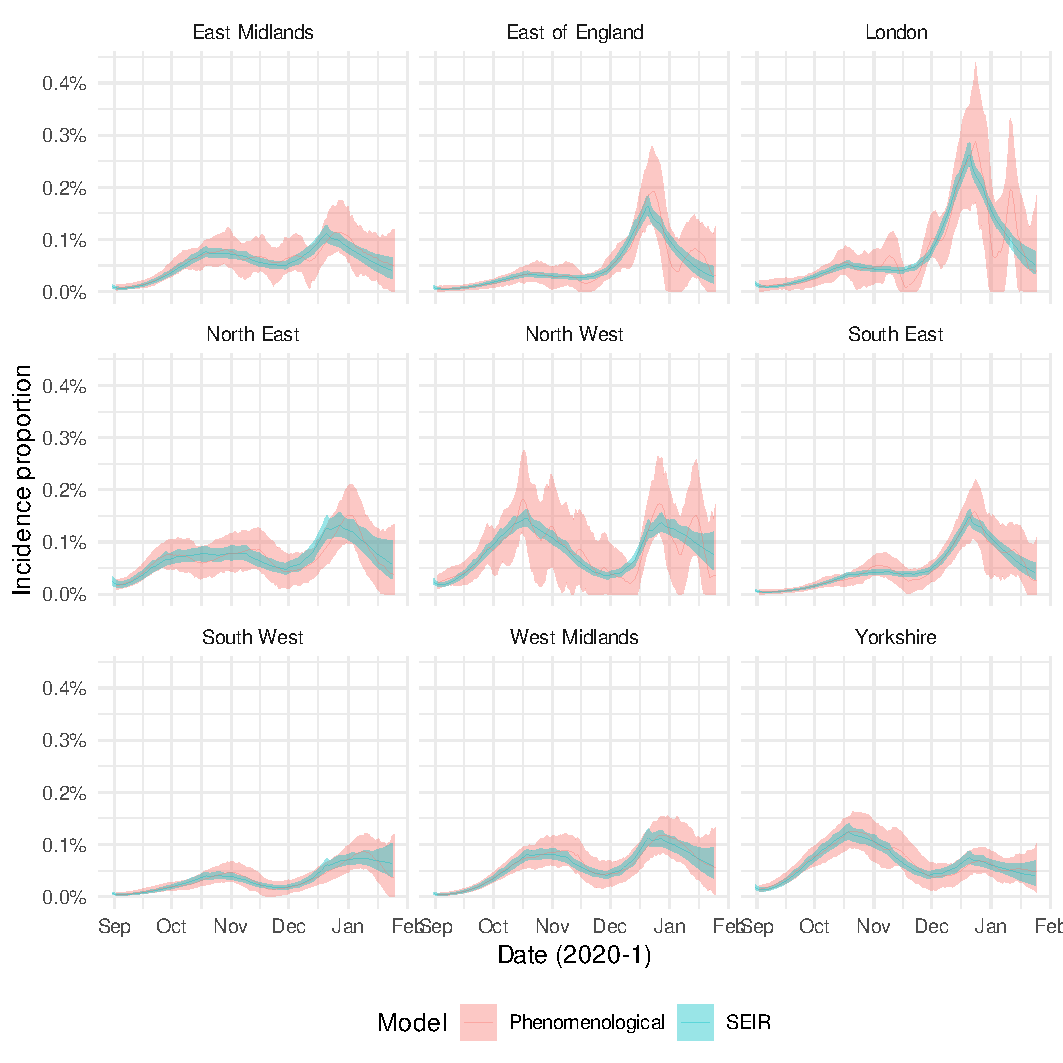
\includegraphics{transmission/compare-regions}
    \caption[Comparing each models estimate of regional incidence.]{%
        Incidence proportion in England and each region estimated by the two models discussed in this chapter.
        Posterior median and 95\% CrI shown.
        For the SEIR model, newly RT-PCR positive (entrances into the P1 compartment), rather than incidence (entrances into the E compartment) are shown for comparability with the backcalculation results.
    }
    \label{transmission:fig:compare-regions}
\end{figure}

These patterns can be interpreted as an instance of the common bias---variance trade-off.
The SEIR model imposes stronger assumptions about the epidemic dynamics.
The assumptions reduces the variance of the estimates, including by making them smoother, but if the assumptions are incorrect, bias is introduced.
Furthermore, the SEIR model does not fully adjust for the non-response bias.
In particular, it makes no adjustment for the under-representation of ethnic minority groups in the CIS.
Adjusting for more covariates would require further stratifying the population, and finding an appropriate parameterisation of the contact matrix.
This trade-off based on the strength of assumptions has long been known to apply in the backcalulcation context~\autocite[e.g.][section 8.3]{brookmeyerBackcalculation}.
The SEIR model can be viewed as a backcalulation method where the transmisson part of the model is a smoothing method.

The backcalculation method benefits from being able to be implemented in a fast, approximate inference package (R-INLA) that easily scales to many parameters, including random effects.
Therefore, it is far more flexible and can easily include time-varying effects, ethnicity, etc.
The SEIR model is limited by the inference procedure and the requirement to sovle an ODE to evaluate the likelihood.
To incorporate a more flexible model, and reduce its bias, a more efficient inference procedure would be required.

Many of these issues are clearly demonstrated by the estimates for the North East (see \cref{transmission:fig:compare-NE}).
I previously observed the quality of the SEIR model's fit is variable between different age groups (see \cref{SEIR:fig:prev-young,SEIR:fig:prev-old}).
This is because the model is not flexible enough to capture the true age distribution of infections.
The overestimation of prevalence in the 11--16 age group and underestimation in the 16--25 age group is reflected when comparing incidence estimates to those from the backcalculation model, which have reduced bias.
\begin{figure}
    \centering 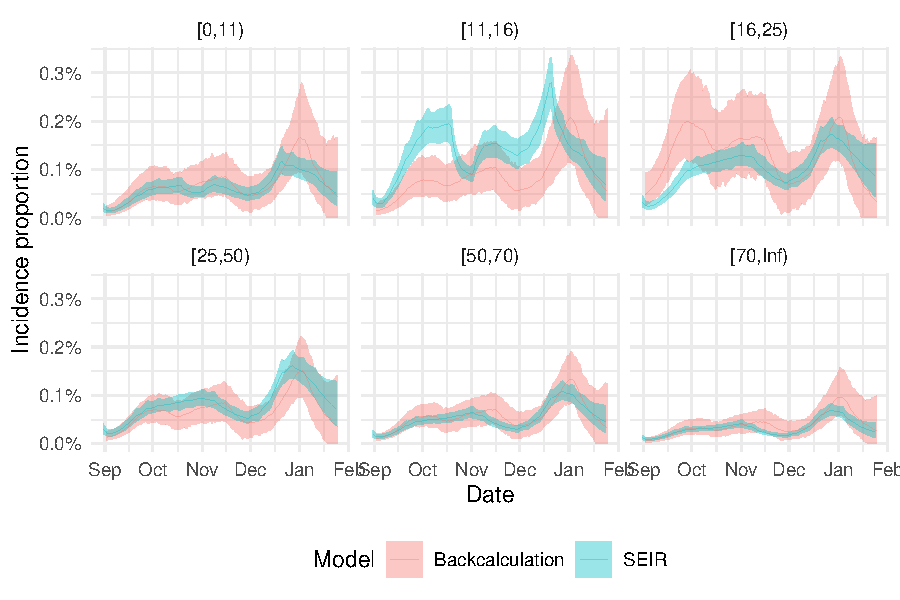
\includegraphics{transmission/compare-NE}
    \caption[Comparing each models estimate of North East incidence by age.]{%
        Incidence proportion in each age group in the North East estimated by the two models discussed in this chapter.
        Posterior median and 95\% CrI shown.
        For the SEIR model, newly RT-PCR positive (entrances into the P1 compartment), rather than incidence (entrances into the E compartment) are shown for comparability with the backcalculation results.
    }
    \label{transmission:fig:compare-NE}
\end{figure}


\section{Conclusion}

The major contribution in this chapter is showing that transmission and incidence can be estimated using only data from the CIS.
A similar survey could, therefore, be considered as the primary form of surveillance for a future pandemic.
The advantage of such a setup is the unbiased information across the entire population, including children.

The transmission model presented in this chapter could be extended to fully extract the information in the CIS (see \cref{SEIR:sec:discussion}).
This would require a more flexible model, which would likely require a more efficient inference procedure, such as NUTS.

\ifSubfilesClassLoaded{
  \appendix
  \subfile{transmission-appendix-INLA}
  \subfile{transmission-appendix-phase-type}
  \listoftodos
}{}

\end{document}